% Phase 1 presentation, M.Tech. Project, Suhas H, roll number 25M0328, CSRE, IIT Bombay.
% Main file. The theme lives in theme.tex.
% Compile from the ppt/ folder of the repository, so that ../figures/ resolves.
% Every number on a slide comes from the Phase 1 report; the registry key behind each
% is named in a comment beside the frame and collected in the table at the end.

\documentclass[aspectratio=169,10pt,t,usepdftitle=false]{beamer}
% Slide theme for the Phase 1 presentation, Suhas H, roll number 25M0328, CSRE, IIT Bombay.
% Replicates the layout of beamer-theme-standard.pdf: white frames, bold blue frame
% titles at the left, the section name at the top, small square bullets; Palatino.
% Three levels, each in its own style: the header (section name, small grey, above a
% hairline), the heading (frame title, large bold blue), the content (black text).
% The footer carries the project title at the left and the two logos at the right.
% Compile from the ppt/ folder of the repository, so that ../figures/ resolves.

% ---------------------------------------------------------------------------
% Type: Palatino, as in the report
% ---------------------------------------------------------------------------
\usepackage[T1]{fontenc}
\usepackage{palatino}
\usefonttheme{serif}
\usefonttheme{professionalfonts}
\usepackage{microtype}

\usepackage{graphicx}
\graphicspath{{../figures/}{../report/}{./}}
\usepackage{booktabs}
\usepackage{array}
\newcolumntype{L}[1]{>{\raggedright\arraybackslash}p{#1}}
\usepackage{tikz}
\usetikzlibrary{positioning,arrows.meta,calc}

% Subscripts in chemical formulae, in the text typeface: SO\sub{2}
\newcommand{\sub}[1]{\textsubscript{#1}}

% ---------------------------------------------------------------------------
% Colours: one blue, the blue of the institute logo, and the theme's orange
% for the rare emphasised word
% ---------------------------------------------------------------------------
\definecolor{iitblue}{HTML}{014EA0}
\definecolor{navy}{HTML}{1A2744}
\definecolor{emph}{HTML}{E08A00}
\definecolor{textcol}{HTML}{111111}
\definecolor{softgrey}{HTML}{6B6B6B}

\setbeamercolor{normal text}{fg=textcol,bg=white}
\setbeamercolor{structure}{fg=iitblue}
\setbeamercolor{frametitle}{fg=iitblue}
\setbeamercolor{title}{fg=iitblue}
\setbeamercolor{item}{fg=iitblue}
\setbeamercolor{alerted text}{fg=emph}
\setbeamercolor{caption name}{fg=iitblue}
\setbeamercolor{block title}{fg=white,bg=iitblue}
\setbeamercolor{block body}{fg=textcol,bg=iitblue!6}

\setbeamerfont{frametitle}{size=\Large,series=\bfseries}
\setbeamerfont{title}{size=\huge,series=\bfseries}
\setbeamerfont{alerted text}{series=\bfseries}
\setbeamerfont{caption}{size=\small}

\setbeamertemplate{navigation symbols}{}
\setbeamertemplate{itemize item}{\small\raise0.25ex\hbox{\vrule width0.55em height0.55em}}
\setbeamertemplate{itemize subitem}{\scriptsize\raise0.3ex\hbox{\vrule width0.5em height0.5em}}
\setbeamertemplate{enumerate item}{\insertenumlabel.}
\setbeamertemplate{blocks}[default]
\setbeamertemplate{caption}[numbered]
\setbeamersize{text margin left=7mm, text margin right=7mm}

% ---------------------------------------------------------------------------
% Header: the current section name, small and grey, at the left above a hairline
% that runs the full text width. It names where the talk is, not the slide.
% ---------------------------------------------------------------------------
\definecolor{hairline}{HTML}{C9CDD4}
\setbeamertemplate{headline}{%
  \vskip2mm
  \hbox to \paperwidth{\hskip7mm
    {\scriptsize\color{softgrey}\insertsectionhead}\hfill}%
  \vskip1.2mm
  \hbox to \paperwidth{\hskip7mm{\color{hairline}\rule{\dimexpr\paperwidth-14mm\relax}{0.4pt}}\hfill}%
}

% ---------------------------------------------------------------------------
% Heading: the frame title, large, bold and blue, at the left. There is no
% subtitle: what the slide shows is said in the content, in black.
% ---------------------------------------------------------------------------
\setbeamertemplate{frametitle}{%
  \vskip3.5mm
  {\usebeamerfont{frametitle}\usebeamercolor[fg]{frametitle}\raggedright
   \insertframetitle\par}%
  \vskip1mm
}

% The one sentence that says what a figure shows: content, so black and upright
\newcommand{\finding}[1]{{\raggedright #1\par}\vskip2mm}

% Literature behind a slide, small and grey at the foot of the content
\newcommand{\refline}[1]{\par\vfill{\raggedright\scriptsize\color{softgrey}#1\par}\vskip0.5mm}

% A small bold blue label that opens a column or a group of points

% Harvey ball: 0 empty, 1 quarter, 2 half, 3 three quarters, 4 full
\newcommand{\hb}[1]{\tikz[baseline=-0.7ex]{%
  \ifcase#1\relax
  \or\fill[iitblue] (0,0) -- (0,1.15mm) arc[start angle=90,end angle=0,radius=1.15mm] -- cycle;%
  \or\fill[iitblue] (0,0) -- (0,1.15mm) arc[start angle=90,end angle=-90,radius=1.15mm] -- cycle;%
  \or\fill[iitblue] (0,0) -- (0,1.15mm) arc[start angle=90,end angle=-180,radius=1.15mm] -- cycle;%
  \or\fill[iitblue] (0,0) circle (1.15mm);%
  \fi
  \draw[iitblue,line width=0.5pt] (0,0) circle (1.15mm);}}
\newcommand{\colhead}[1]{{\bfseries\color{iitblue}#1\par}\vskip1mm}

% Drawn diagrams: flat boxes with a thin blue border, plain arrows
\tikzset{
  box/.style={draw=iitblue,line width=0.6pt,fill=iitblue!5,align=center,
              inner sep=1.8mm,font=\small,text width=#1,minimum height=11mm},
  box/.default={24mm},
  keybox/.style={box=#1,fill=iitblue,text=white,font=\small\bfseries},
  keybox/.default={24mm},
  greybox/.style={box=#1,draw=softgrey,fill=black!4,text=softgrey},
  greybox/.default={24mm},
  flow/.style={-{Stealth[length=2.2mm]},line width=0.7pt,color=iitblue},
  note/.style={font=\scriptsize,text=softgrey,align=center}}

% Outline: numbered sections in blue
\setbeamertemplate{section in toc}{%
  {\color{iitblue}\bfseries\inserttocsectionnumber.}\hskip2mm\inserttocsection\par}
\setbeamerfont{section in toc}{size=\large}

% ---------------------------------------------------------------------------
% Foot: the project title at the left, the two logos small at the right
% ---------------------------------------------------------------------------
\newcommand{\footlogoheight}{4.8mm}
\setbeamertemplate{footline}{%
  \hbox to \paperwidth{%
    \hskip7mm
    \raisebox{1.1mm}{\tiny\bfseries\color{iitblue}\insertshorttitle}%
    \hfill
    
\includegraphics[height=\footlogoheight]{iitb-logo}%
    \hskip2.5mm
    
\includegraphics[height=\footlogoheight]{csre-logo}%
    \hskip7mm}%
  \vskip2.5mm
}

% ---------------------------------------------------------------------------
% Title page: the two logos at the same height, mirrored about the centre line
% of the page and level with the title; below, the lines of the report's title
% page, one under the other, centred
% ---------------------------------------------------------------------------
% The CSRE mark is about twice as wide as the IIT Bombay seal, so at equal height it
% looks heavier; it is set a little smaller. Each logo is placed from the edge of
% the title itself, at the same gap, so the title sits exactly between them; the
% logos and the title block share one vertical centre.
\newcommand{\titlelogoheight}{13mm}
\newcommand{\csrelogoheight}{10.5mm}
\newcommand{\logogap}{12.8mm}
\newcommand{\talksubtitle}{}
\newcommand{\talkdetails}{}
\newcommand{\maketitleframe}{%
  \begin{frame}[plain,noframenumbering]
    \begin{tikzpicture}[remember picture,overlay]
      \node[anchor=center,align=center,inner sep=0pt] (titleblock)
        at ([yshift=-15mm]current page.north)
        {{\usebeamerfont{title}\usebeamercolor[fg]{title}\inserttitle}\\[1mm]
         {\small\talksubtitle}};
      \node[anchor=east,inner sep=0pt]
        at ([xshift=-\logogap]titleblock.west)
        {
\includegraphics[height=\titlelogoheight]{iitb-logo}};
      \node[anchor=west,inner sep=0pt]
        at ([xshift=\logogap]titleblock.east)
        {
\includegraphics[height=\csrelogoheight]{csre-logo}};
      \node[anchor=north,text width=0.84\paperwidth,align=center,inner sep=0pt]
        at ([yshift=-33mm]current page.north)
        {\talkdetails};
    \end{tikzpicture}
  \end{frame}
}

% ---------------------------------------------------------------------------
% Closing frame: the words alone, at the exact centre of the page, large, bold, navy
% ---------------------------------------------------------------------------
\newcommand{\makeclosingframe}[1]{%
  \begin{frame}[plain,noframenumbering,c]
    \begin{tikzpicture}[remember picture,overlay]
      \node[anchor=center,inner sep=0pt] at (current page.center)
        {\fontsize{30}{34}\selectfont\bfseries\color{navy}#1};
    \end{tikzpicture}
  \end{frame}
}


\usepackage[english]{babel}
\hypersetup{pdftitle={Venus Photochemistry},pdfauthor={Suhas H}}

\title[Venus Photochemistry]{Venus Photochemistry}
\renewcommand{\talksubtitle}{M.Tech.\ Project, Phase 1 Presentation}
\renewcommand{\talkdetails}{%
  % The lines of the report's title page, from the name down, in the same order
  {\large\bfseries Suhas H\par}
  \vskip0.6mm
  {\small Roll Number: 25M0328\par}
  \vskip2mm
  {\small Under the Supervision of\par}
  \vskip0.6mm
  {\large\bfseries Prof.\ Deepak Singh\par}
  \vskip2.5mm
  {\small Geoinformatics and Natural Resources Engineering\par}
  \vskip0.4mm
  {\small Centre of Studies in Resources Engineering\par}
  \vskip2.5mm
  {\normalsize\bfseries INDIAN INSTITUTE OF TECHNOLOGY BOMBAY\par}
  \vskip0.8mm
  {\small\bfseries Mumbai -- 400076, India\par}}

\begin{document}

\maketitleframe

\begin{frame}{Outline}
  \vskip4mm
  \tableofcontents
\end{frame}

% ===========================================================================
\section{Introduction}
% ===========================================================================

% Slide 1. Report Section 1.1, Figure F01. Literature: Dai et al. (2025).
% Band: e6.interval.90.lo and .hi.
\begin{frame}{Venus and its clouds}
  \begin{columns}[T,onlytextwidth]
    \begin{column}{0.52\textwidth}
      \centering
      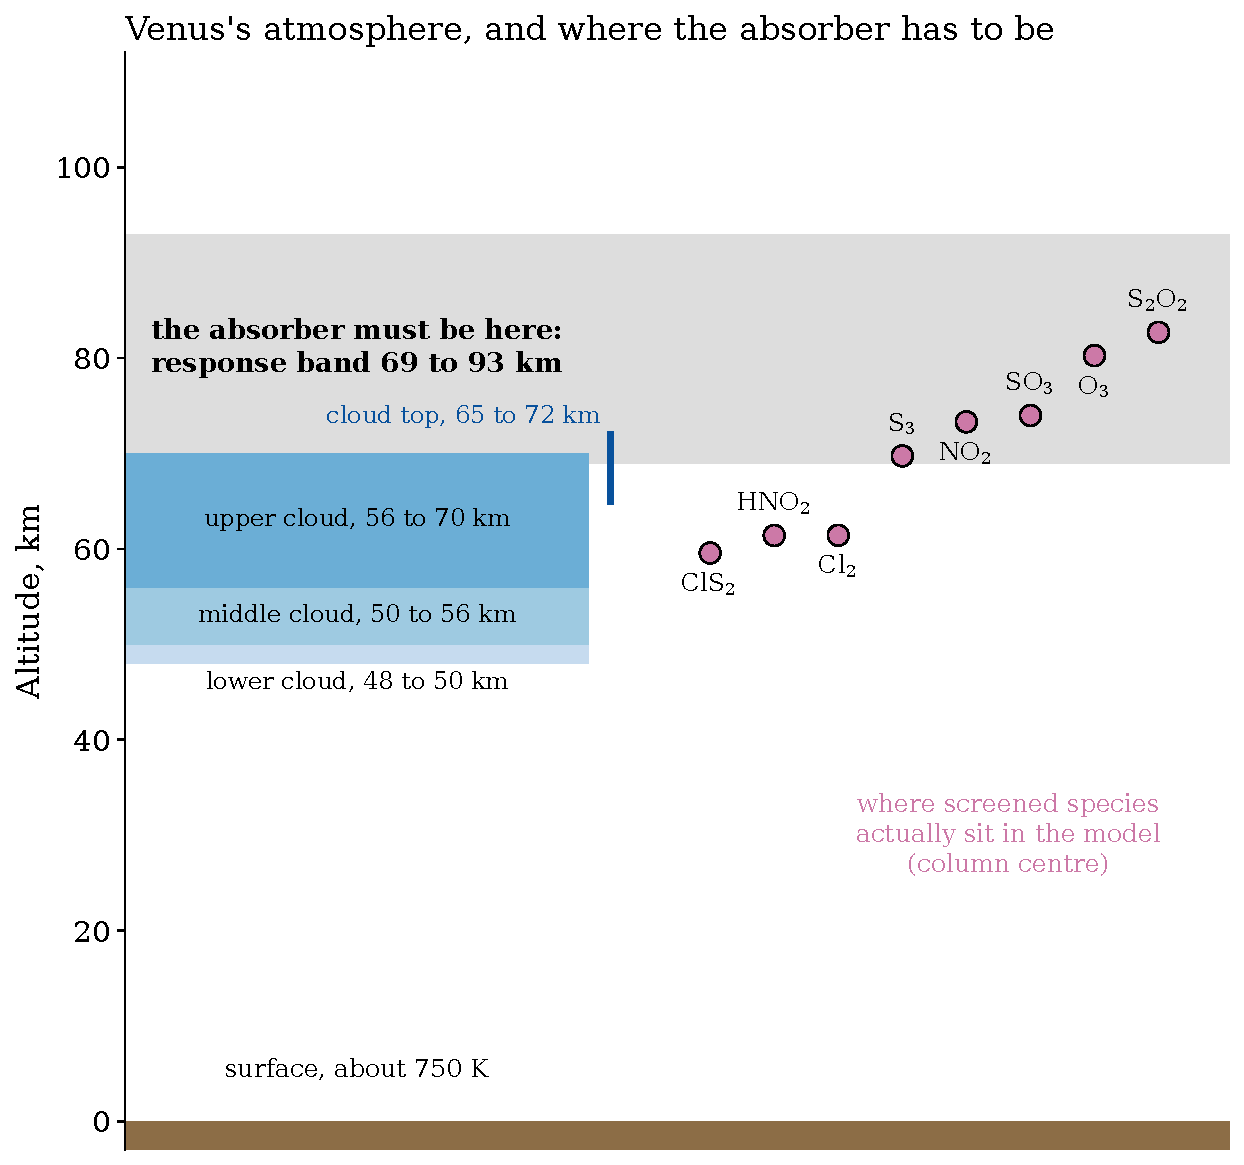
\includegraphics[height=0.74\textheight]{F01_CTX_venus-atmosphere_ch1_s3.pdf}
    \end{column}
    \begin{column}{0.45\textwidth}
      \vskip8mm
      \begin{itemize}\setlength{\itemsep}{4mm}
        \item Surface: 92 bar, about 750 K.
        \item Sulfuric acid clouds, 47 to about 70 km.
        \item Cloud top: 65 to 72 km.
        \item Grey band: where the model responds, 69 to 93 km.
      \end{itemize}
    \end{column}
  \end{columns}
  \refline{Dai et al.\ (2025)}
\end{frame}

% Slide 2. Report Section 1.2, Figure F02.
% Literature: Perez-Hoyos et al. (2018); Dai et al. (2025); Titov et al. (2008).
\begin{frame}{The unknown ultraviolet absorber}
  \begin{columns}[T,onlytextwidth]
    \begin{column}{0.58\textwidth}
      \centering
      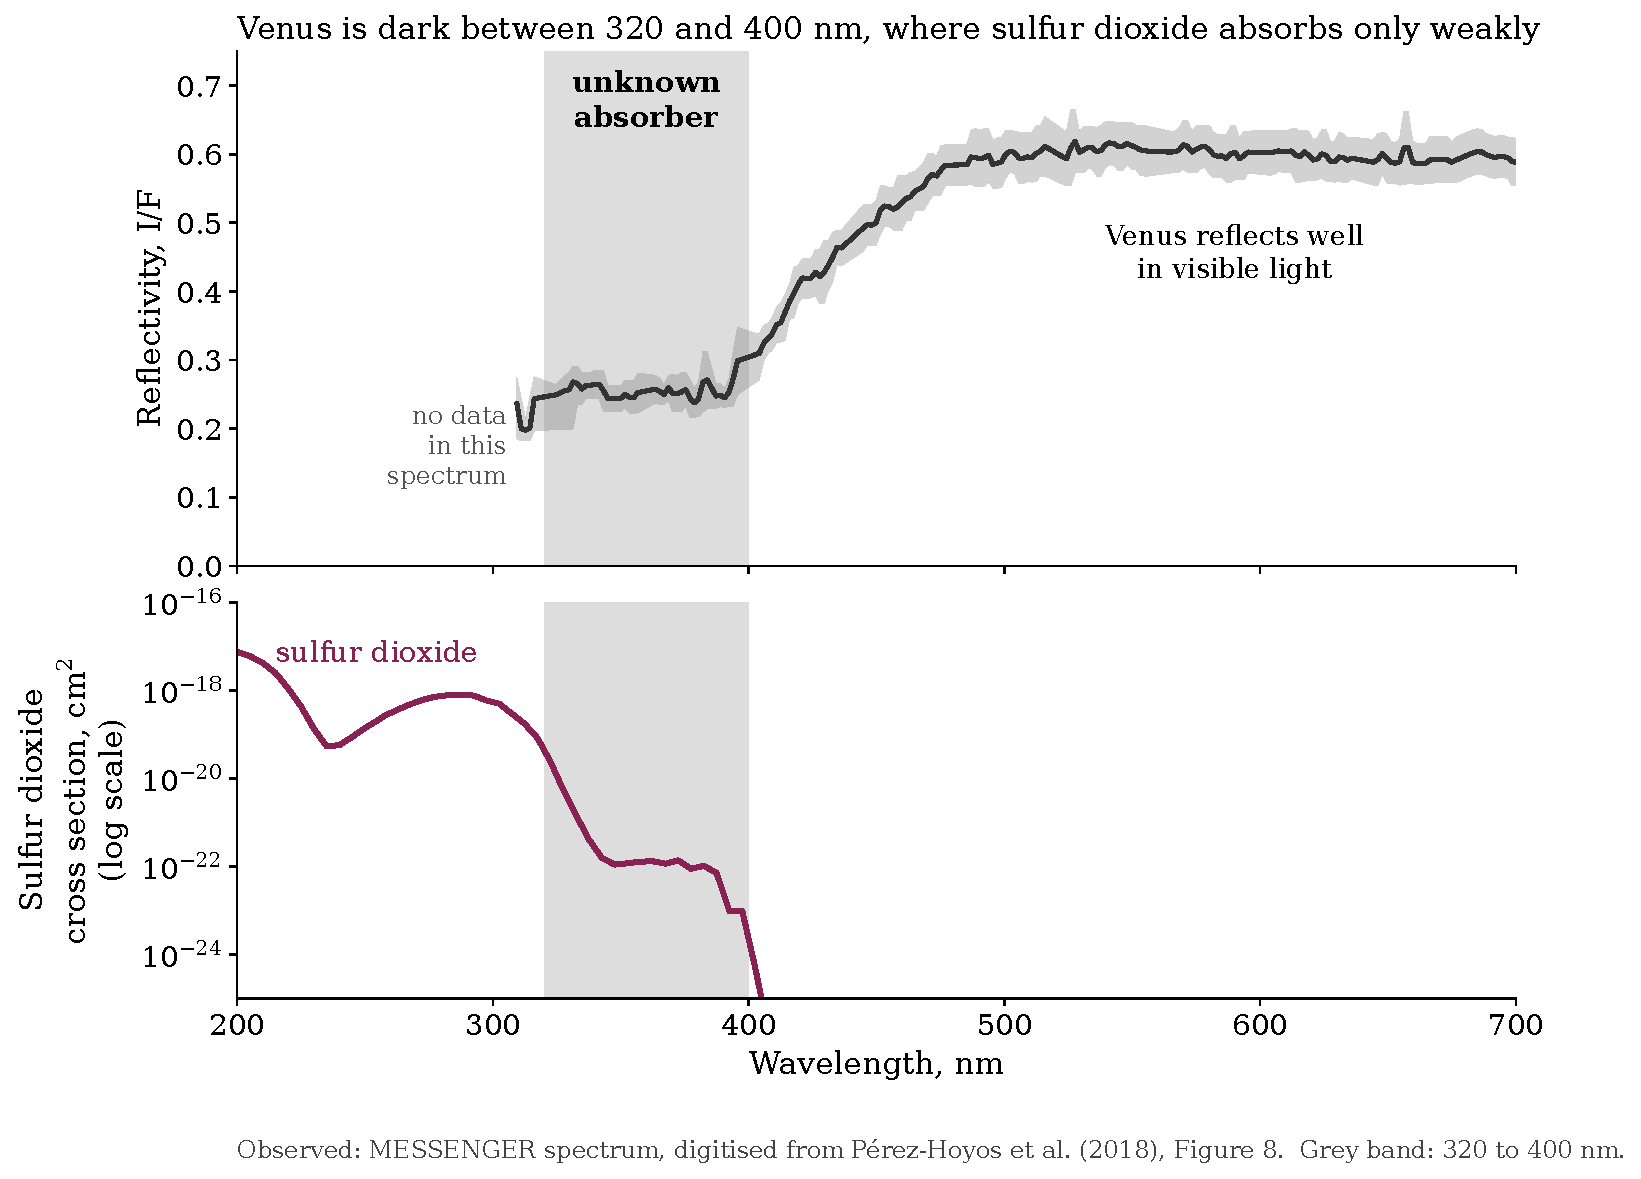
\includegraphics[width=\linewidth,height=0.72\textheight,keepaspectratio]{F02_CTX_observed-uv-absorption_ch1_s2.pdf}
    \end{column}
    \begin{column}{0.39\textwidth}
      \vskip8mm
      \begin{itemize}\setlength{\itemsep}{4mm}
        \item Dark at 320 to 400 nm; SO\sub{2} cannot explain it.
        \item About half the solar heating at the cloud top.
        \item Amount varied twofold, 2006 to 2017.
        \item Its markings trace vertical motion.
      \end{itemize}
    \end{column}
  \end{columns}
  \refline{P\'erez-Hoyos et al.\ (2018); Dai et al.\ (2025); Titov et al.\ (2008)}
\end{frame}

% Slide 3. Report Section 1.3, Table 1.1, cut down.
\begin{frame}{The candidates proposed so far}
  \vskip1mm
  \centering
  \small
  \renewcommand{\arraystretch}{1.08}
  \begin{tabular}{@{}lll@{}}
    \toprule
    \textbf{Candidate} & \textbf{For} & \textbf{Against}\\
    \midrule
    Sulfur dioxide, SO\sub{2}        & Matches below 320 nm        & Negligible beyond 320 nm\\
    Polysulfur, S\sub{x}             & Early spectral candidate    & No form matches\\
    Ferric chloride, FeCl\sub{3}     & Dissolves in the acid       & Band too narrow and weak\\
    Disulfur monoxide, S\sub{2}O     & Matches 400 to 500 nm       & Fades at 320 to 340 nm\\
    OSSO, S\sub{2}O\sub{2}           & Matches 330 to 420 nm       & Far too little at cloud top\\
    Iron and sulfur minerals         & Absorb at 300 to 500 nm     & Presence unknown\\
    Chlorine and sulfur compounds    & Spectra close               & No abundance given\\
    Organic ``red oil''             & Dissolves in acid           & Speculative\\
    A mixture of absorbers           & Explains the band's width   & Not yet tested\\
    \bottomrule
  \end{tabular}
  \vskip2mm
  \finding{Almost every case rests on the spectrum alone.}
  \refline{Dai et al.\ (2025); P\'erez-Hoyos et al.\ (2018)}
\end{frame}

% Literature survey. Report Chapter 2, one row per paper reviewed (12).
% Shading rests on each section's Results and Critique and on Section 2.11.
\begin{frame}{Literature survey: twelve papers, three tests}
  \begin{columns}[T,onlytextwidth]
    \begin{column}{0.74\textwidth}
      \footnotesize
      \setlength{\tabcolsep}{4.5pt}
      \renewcommand{\arraystretch}{0.96}
      \begin{tabular}{@{}llccc@{}}
        \toprule
        \textbf{Paper} & \textbf{Focus} & \textbf{Spectrum} & \textbf{Amount} & \textbf{Altitude}\\
        \midrule
        Dai et al.\ (2024)            & The model, OSSO          & \hb1 & \hb2 & \hb1\\
        P\'erez-Hoyos et al.\ (2018)  & Observed absorber        & \hb2 & \hb0 & \hb1\\
        Bierson and Zhang (2020)      & Mixing, OSSO             & \hb1 & \hb2 & \hb2\\
        Rimmer et al.\ (2021)         & Droplet chemistry        & \hb2 & \hb1 & \hb1\\
        Lef\`evre et al.\ (2022)       & Cloud convection        & \hb0 & \hb1 & \hb0\\
        Lef\`evre et al.\ (2024)       & With chemistry          & \hb0 & \hb0 & \hb0\\
        Jiang et al.\ (2024)          & Iron sulfates            & \hb2 & \hb2 & \hb0\\
        Trabelsi and Francisco (2026) & Chlorine and sulfur      & \hb2 & \hb0 & \hb0\\
        Egan et al.\ (2025)           & OSSO, end to end         & \hb4 & \hb4 & \hb2\\
        Spacek et al.\ (2026)         & Strength needed          & \hb2 & \hb4 & \hb1\\
        Egan, James and Plane (2025)  & FeCl\sub{3}, laboratory  & \hb2 & \hb0 & \hb0\\
        Egan et al.\ (2026)           & FeCl\sub{3}, 3D model    & \hb4 & \hb2 & \hb1\\
        \midrule
        \textbf{This project}         & \textbf{All in one model} & \hb2 & \hb2 & \hb4\\
        \bottomrule
      \end{tabular}
    \end{column}
    \begin{column}{0.23\textwidth}
      \colhead{Key}
      \footnotesize
      \renewcommand{\arraystretch}{1.5}
      \begin{tabular}{@{}cl@{}}
        \hb0 & Not addressed\\
        \hb1 & Assumed or set\\
        \hb2 & Partly tested\\
        \hb4 & Tested in full\\
      \end{tabular}
      \vskip3mm
      {\scriptsize\color{softgrey}Partly: shape only, an estimate, or no light calculation.\par
      Full: absolute, against observation.\par
      \vskip2mm
      The twelve papers reviewed; five more references are background.\par}
    \end{column}
  \end{columns}
  \vskip2mm
  \finding{In the literature, altitude is never tested in full: it is assumed, set, or left out.}
\end{frame}

% Slide 5. Report Sections 1.4, 1.5 and 2.11.
\begin{frame}{Research gap and objective}
  \finding{Gap: no study lets a model place a candidate and measures the effect of where it sits.}
  \vskip3mm
  \centering
  \colhead{This project: all three tests at once, inside one model}
  \vskip3mm
  % One size for every box: 24 mm wide, 14 mm tall, three short lines each
  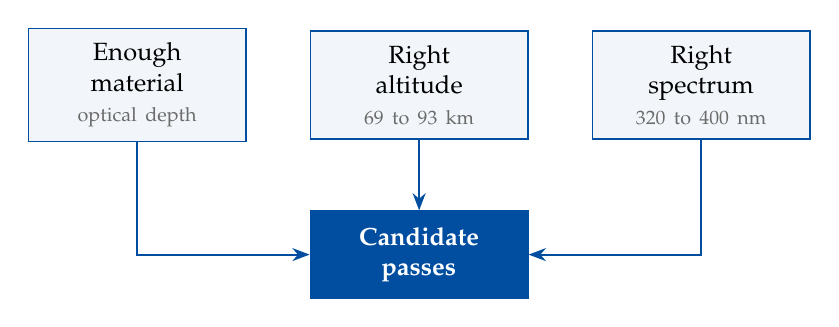
\begin{tikzpicture}[node distance=8mm,
      every node/.append style={minimum height=14mm}]
    \node[box=24mm] (a) {Enough\\material\\{\scriptsize\color{softgrey}optical depth}};
    \node[box=24mm, right=of a] (b) {Right\\altitude\\{\scriptsize\color{softgrey}69 to 93 km}};
    \node[box=24mm, right=of b] (c) {Right\\spectrum\\{\scriptsize\color{softgrey}320 to 400 nm}};
    \node[keybox=24mm, below=9mm of b] (d) {Candidate\\passes};
    \draw[flow] (a.south) |- (d.west);
    \draw[flow] (b) -- (d);
    \draw[flow] (c.south) |- (d.east);
  \end{tikzpicture}
\end{frame}

% ===========================================================================
\section{The Model and the Method}
% ===========================================================================

% Slide 5. Report Sections 3.1 to 3.3, Table 3.1.
\begin{frame}{The model: VULCAN-Venus}
  \vskip1mm
  \begin{columns}[T,onlytextwidth]
    \begin{column}{0.50\textwidth}
      \colhead{How an absorber acts on the model}
      \vskip1mm
      \centering
      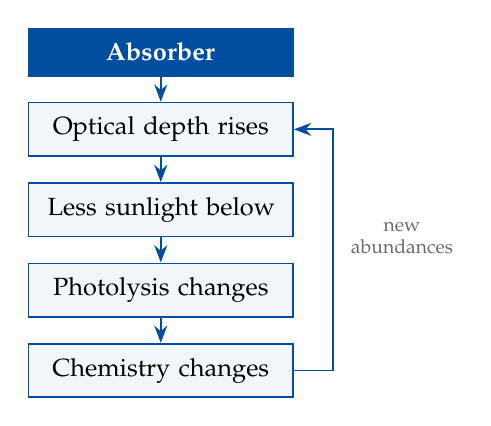
\begin{tikzpicture}[node distance=3.2mm]
        \node[keybox=30mm, minimum height=6mm] (a) {Absorber};
        \node[box=30mm, minimum height=6mm, below=of a] (b) {Optical depth rises};
        \node[box=30mm, minimum height=6mm, below=of b] (c) {Less sunlight below};
        \node[box=30mm, minimum height=6mm, below=of c] (d) {Photolysis changes};
        \node[box=30mm, minimum height=6mm, below=of d] (e) {Chemistry changes};
        \draw[flow] (a) -- (b); \draw[flow] (b) -- (c);
        \draw[flow] (c) -- (d); \draw[flow] (d) -- (e);
        \draw[flow] (e.east) -- ++(5mm,0) |- (b.east);
        \node[note, anchor=west] at ($(c.east)+(6mm,-3.6mm)$) {new\\abundances};
      \end{tikzpicture}
    \end{column}
    \begin{column}{0.47\textwidth}
      \colhead{Set-up of every Phase 1 run}
      \small
      \renewcommand{\arraystretch}{1.25}
      \begin{tabular}{@{}ll@{}}
        \toprule
        Grid        & 0 to 112 km, 57 layers\\
        Chemistry   & 62 entries, 838 reaction slots\\
        Wavelengths & 1670 bins, 96 to 698 nm\\
        Sunlight    & One angle, 58 degrees\\
        Mixing      & Bierson and Zhang\\
        Off         & Vertical wind\\
        \bottomrule
      \end{tabular}
    \end{column}
  \end{columns}
  \refline{Dai, Shao and Sheng (2024); Bierson and Zhang (2020)}
\end{frame}

% Slide 6. Report Sections 3.3 to 3.6.
% Number: const.tau_req = 1.094968472081, printed as 1.095.
\begin{frame}{The groundwork: an absorber that was switched off}
  \vskip4mm
  \centering
  % One size for every box: 25 mm wide, 12 mm tall, two lines each
  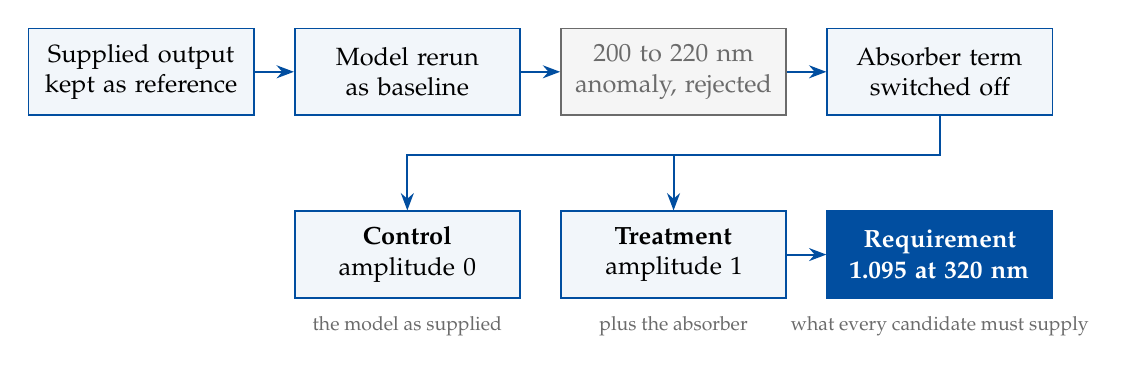
\begin{tikzpicture}[node distance=5mm,
      every node/.append style={minimum height=12mm}]
    \node[box=25mm] (a) {Supplied output\\kept as reference};
    \node[box=25mm, right=of a] (b) {Model rerun\\as baseline};
    \node[greybox=25mm, right=of b] (c) {200 to 220 nm\\anomaly, rejected};
    \node[box=25mm, right=of c] (d) {Absorber term\\switched off};
    \draw[flow] (a) -- (b); \draw[flow] (b) -- (c); \draw[flow] (c) -- (d);
    \node[box=25mm, below=12mm of b] (e) {\textbf{Control}\\amplitude 0};
    \node[box=25mm, below=12mm of c] (f) {\textbf{Treatment}\\amplitude 1};
    \node[keybox=25mm, below=12mm of d] (g) {Requirement\\1.095 at 320 nm};
    \draw[flow] (d.south) -- ++(0,-5mm) -| (e.north);
    \draw[flow] (d.south) -- ++(0,-5mm) -| (f.north);
    \draw[flow] (f) -- (g);
    \node[note, below=1mm of e, minimum height=0pt] {the model as supplied};
    \node[note, below=1mm of f, minimum height=0pt] {plus the absorber};
    \node[note, below=1mm of g, minimum height=0pt] {what every candidate must supply};
  \end{tikzpicture}
  \vskip3mm
  \finding{Control and treatment differ in one term only.}
\end{frame}

% Slide 7. Report Section 3.7, Figure F04.
\begin{frame}{What was done, in four stages}
  \finding{Fourteen experiments; each stage builds on the one before.}
  \centering
  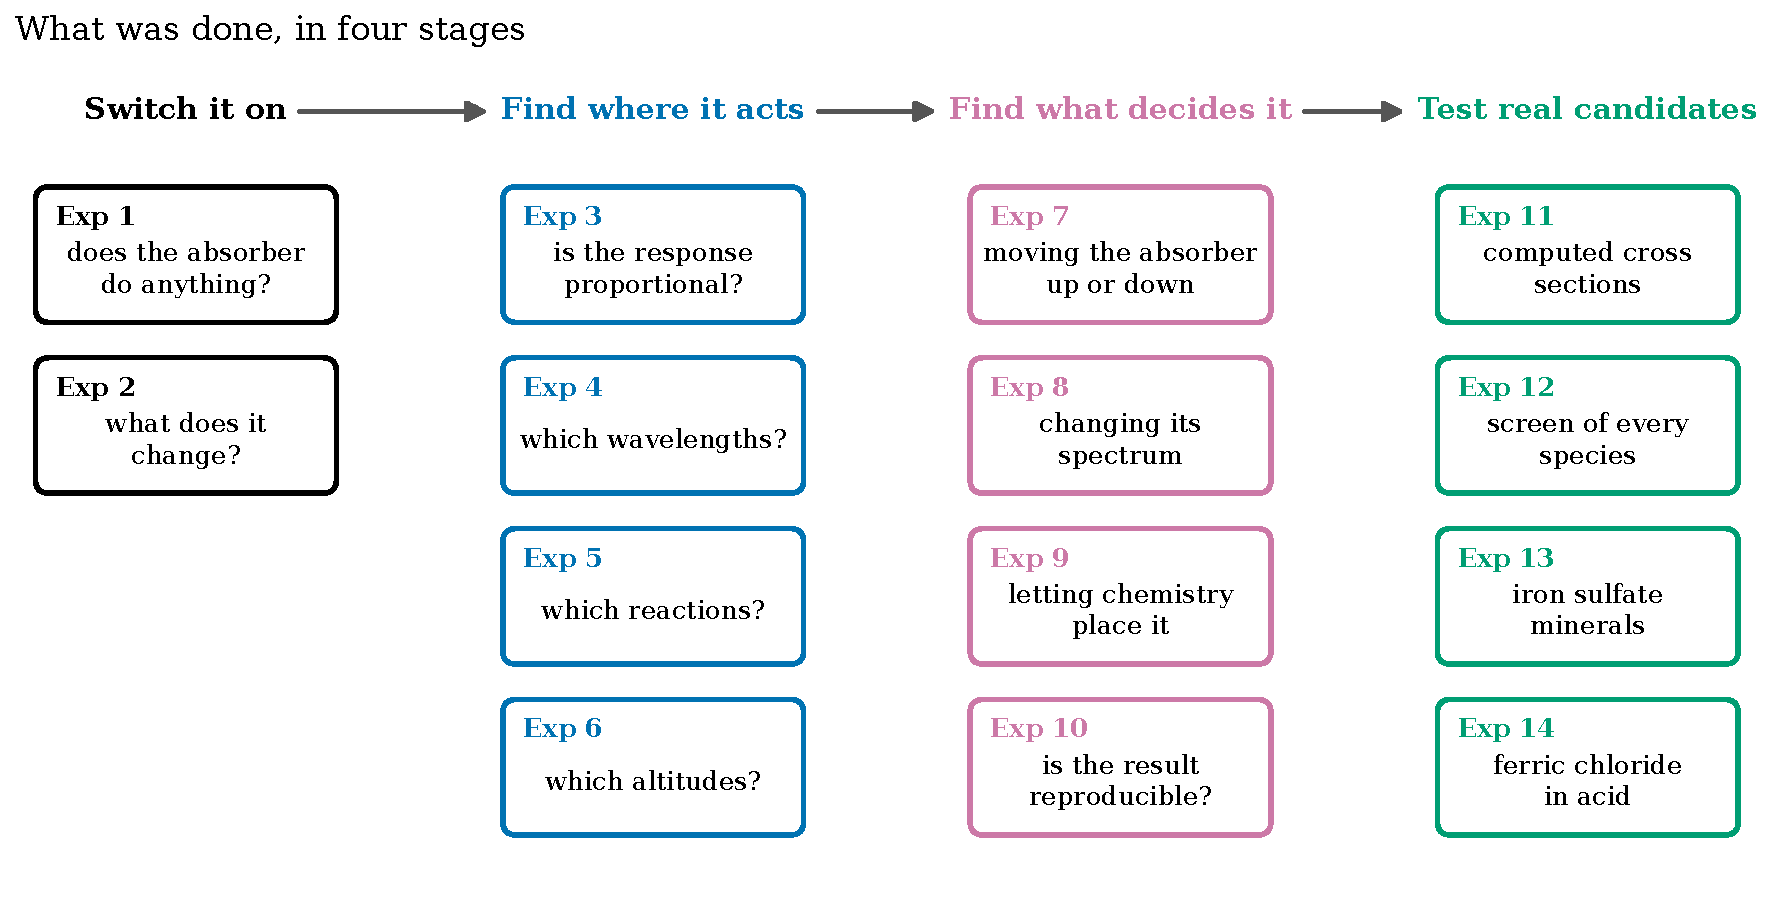
\includegraphics[width=\linewidth,height=0.61\textheight,keepaspectratio]{F04_CTX_what-was-done_ch3_report.pdf}
  \par\vskip1mm
  \raggedright
  \begin{itemize}
    \item Each effect is one number: the change in sunlight, in per cent of the sunlight itself.
  \end{itemize}
\end{frame}

% Slide 9. Report Sections 4.6 and 6.3, Figure F13 (the two floor slides merged).
% Numbers: e10.fielddiff_pct 0.0017; res.e9.SO.inband 0.7384; res.e10.SO.inband 2.5278.
\begin{frame}{How small a change is real}
  \finding{Experiment 10 repeats Experiment 9; the gap between them is numerical noise.}
  \begin{columns}[T,onlytextwidth]
    \begin{column}{0.58\textwidth}
      \centering
      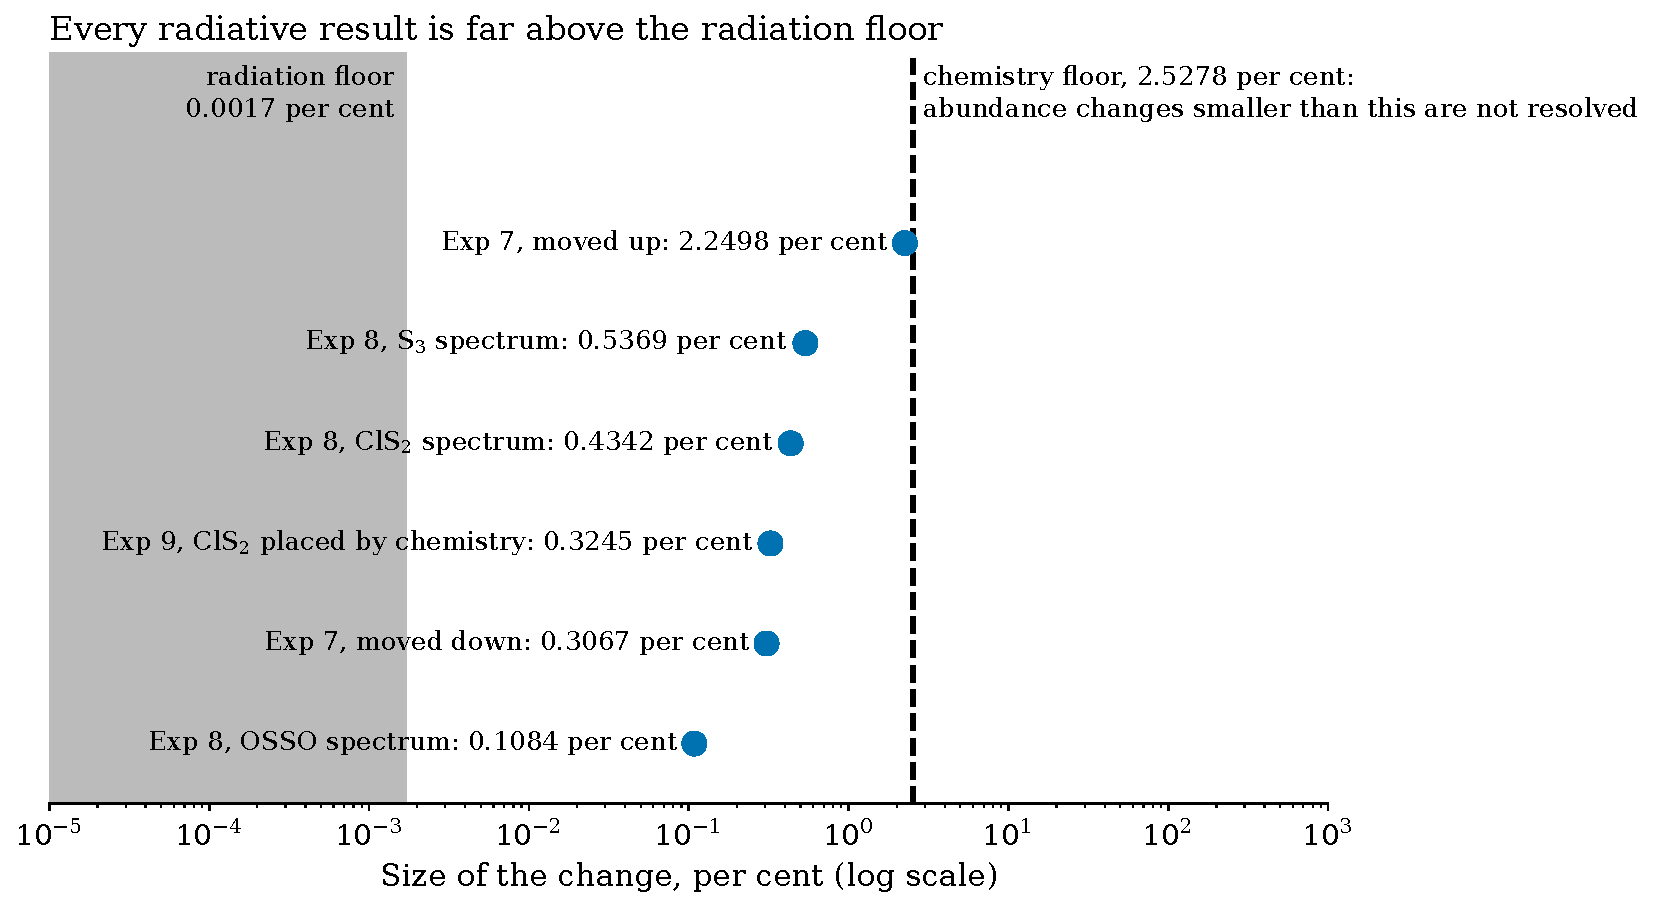
\includegraphics[width=\linewidth,height=0.66\textheight,keepaspectratio]{F13_E10_noise-floors_ch6_backup.pdf}
    \end{column}
    \begin{column}{0.39\textwidth}
      \vskip2mm
      \small
      \begin{itemize}\setlength{\itemsep}{2.5mm}
        \item Sunlight: the runs differ by 0.0017\% of the change. Resolved.
        \item SO in the band: 0.7384\% against 2.5278\%. Noise.
      \end{itemize}
      \vskip3mm
      \begin{block}{The rule}
        Abundance changes below 2.5278\% are upper bounds, not measurements.
      \end{block}
    \end{column}
  \end{columns}
\end{frame}

% ===========================================================================
\section{Experiments 1 to 7}
% ===========================================================================

% Slide 10. Report Section 5.1, Figure F05.
% Numbers: e1.aflux.meanrel 0.013553; e3fp.bnd.A1.aflux.max_pct 87.404;
% e2.SO2.maxrel 0.2243; e2.SO.maxrel 1.7399.
\begin{frame}{Experiments 1 and 2: does the absorber do anything?}
  \finding{Switched on, the absorber changes sunlight strongly and the sulfur species barely.}
  \begin{columns}[T,onlytextwidth]
    \begin{column}{0.58\textwidth}
      \centering
      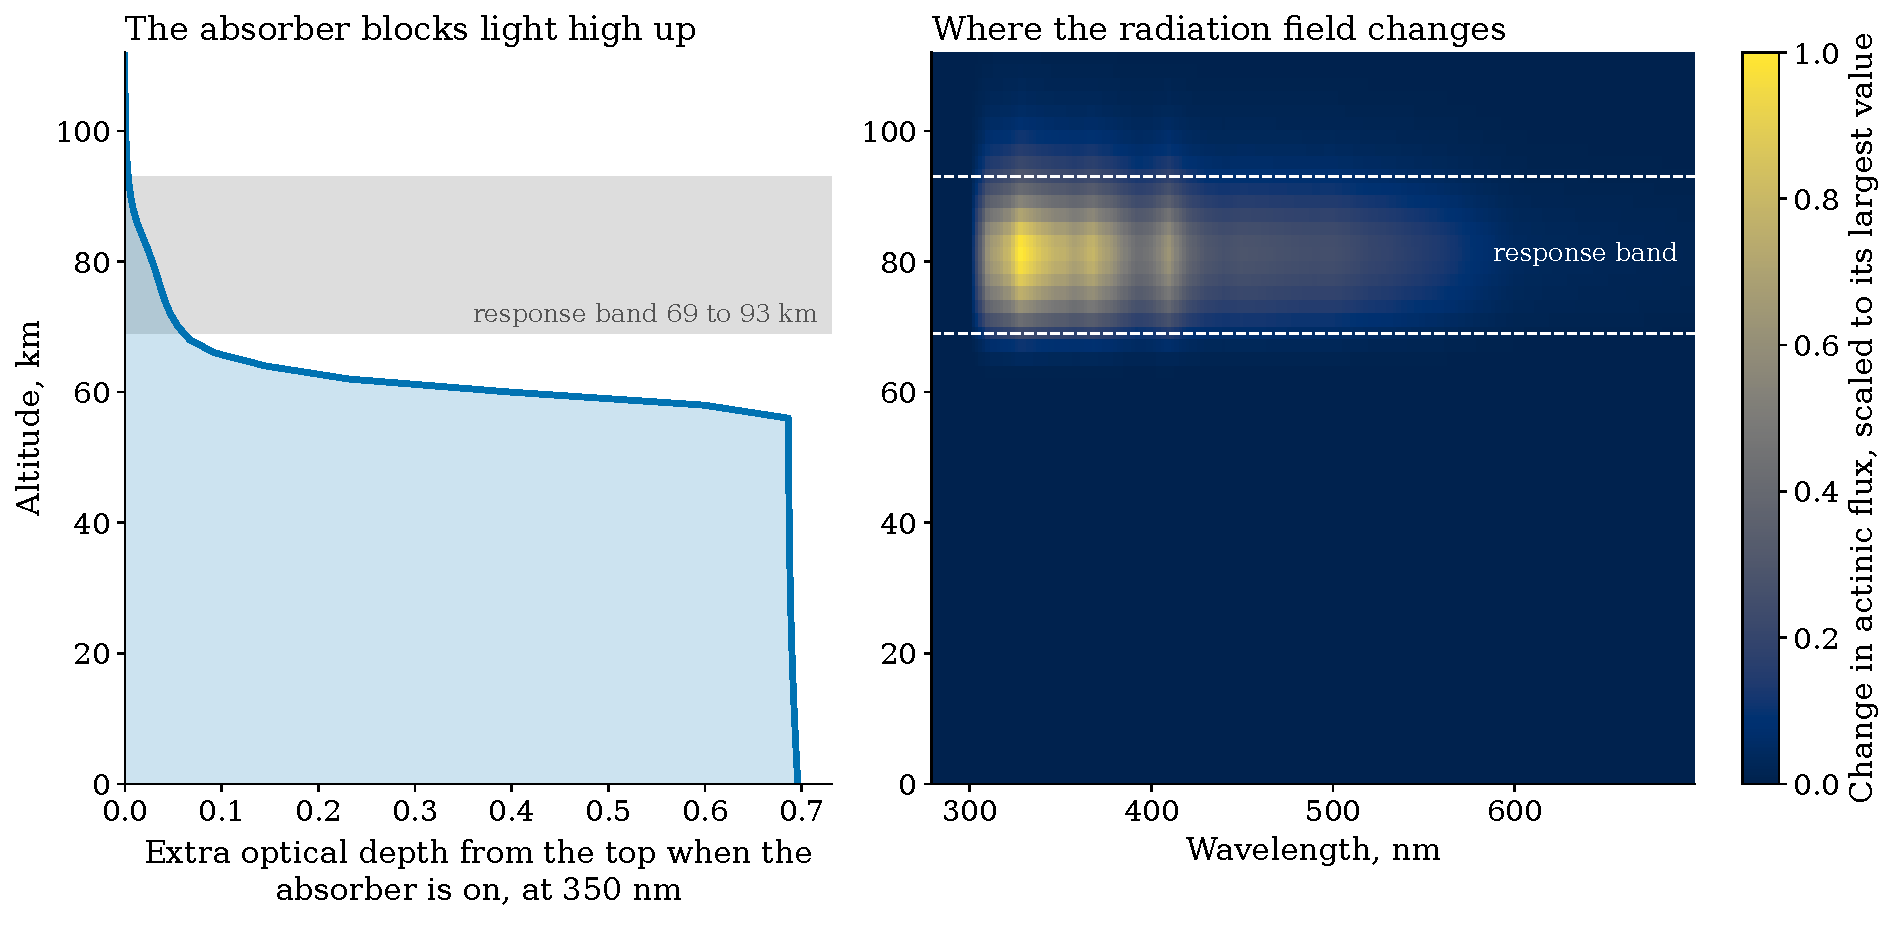
\includegraphics[width=\linewidth,height=0.66\textheight,keepaspectratio]{F05_E01-02_absorber-effect_ch5_s7.pdf}
    \end{column}
    \begin{column}{0.40\textwidth}
      \vskip4mm
      \small
      \renewcommand{\arraystretch}{1.3}
      \begin{tabular}{@{}lrl@{}}
        \toprule
        & Largest change & Verdict\\
        \midrule
        Sunlight & 87.404\% & resolved\\
        SO\sub{2} & 0.2243\% & below floor\\
        SO & 1.7399\% & below floor\\
        \bottomrule
      \end{tabular}
    \end{column}
  \end{columns}
  \refline{Experiment 1: the control matches the supplied model, mean change 0.013553\%.}
\end{frame}

% Slide 11. Report Section 5.2, Figure F06.
% Numbers: e3.lin.tau.inband.median 1.00002; e3.lin.aflux.inband.median 1.00208;
% e3fp.aflux.ratio.A0p5 1.010795; e3fp.aflux.ratio.A2p0 0.979304.
\begin{frame}{Experiment 3: is the response proportional?}
  \begin{columns}[T,onlytextwidth]
    \begin{column}{0.48\textwidth}
      \centering
      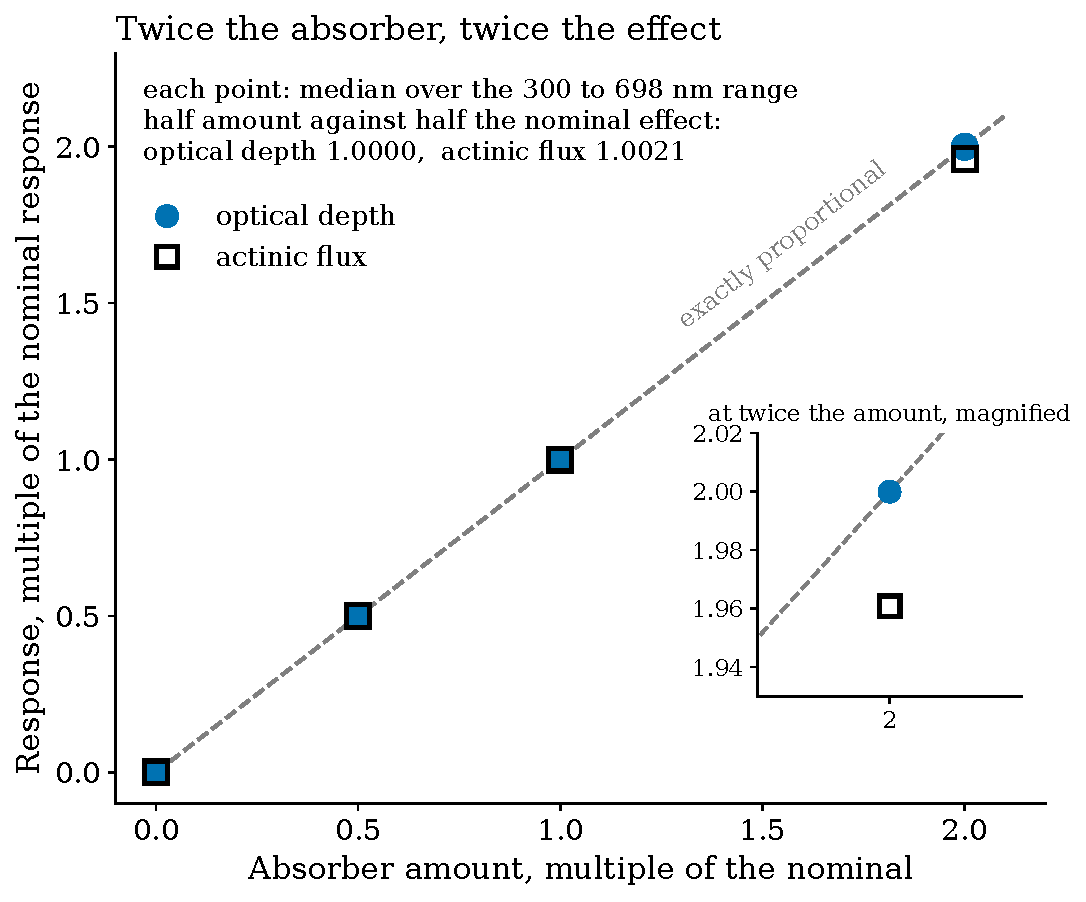
\includegraphics[width=\linewidth,height=0.76\textheight,keepaspectratio]{F06_E03_linear-response_ch5_s8.pdf}
    \end{column}
    \begin{column}{0.49\textwidth}
      \vskip4mm
      \finding{Half, nominal and twice the amount: the response scales with it.}
      \small
      \renewcommand{\arraystretch}{1.25}
      \begin{tabular}{@{}lr@{}}
        \toprule
        Test, where 1 means proportional & Ratio\\
        \midrule
        Optical depth, half amount & 1.00002\\
        Sunlight, half amount & 1.00208\\
        Whole field, half amount & 1.010795\\
        Whole field, twice the amount & 0.979304\\
        \bottomrule
      \end{tabular}
      \vskip4mm
      \normalsize
      \begin{itemize}
        \item Chemistry: within the floor, not resolved.
      \end{itemize}
    \end{column}
  \end{columns}
\end{frame}

% Slide 12. Report Section 5.3, Table 5.1 (four rows), Figure F07.
% Numbers: e4a.S2O_1.300_320.pct 93.689; e4a SO3 300 to 320 80.754;
% e4a S3 380 to 420 49.605; e4a S4 420 to 620 100.
\begin{frame}{Experiment 4: which wavelengths?}
  \begin{columns}[T,onlytextwidth]
    \begin{column}{0.50\textwidth}
      \centering
      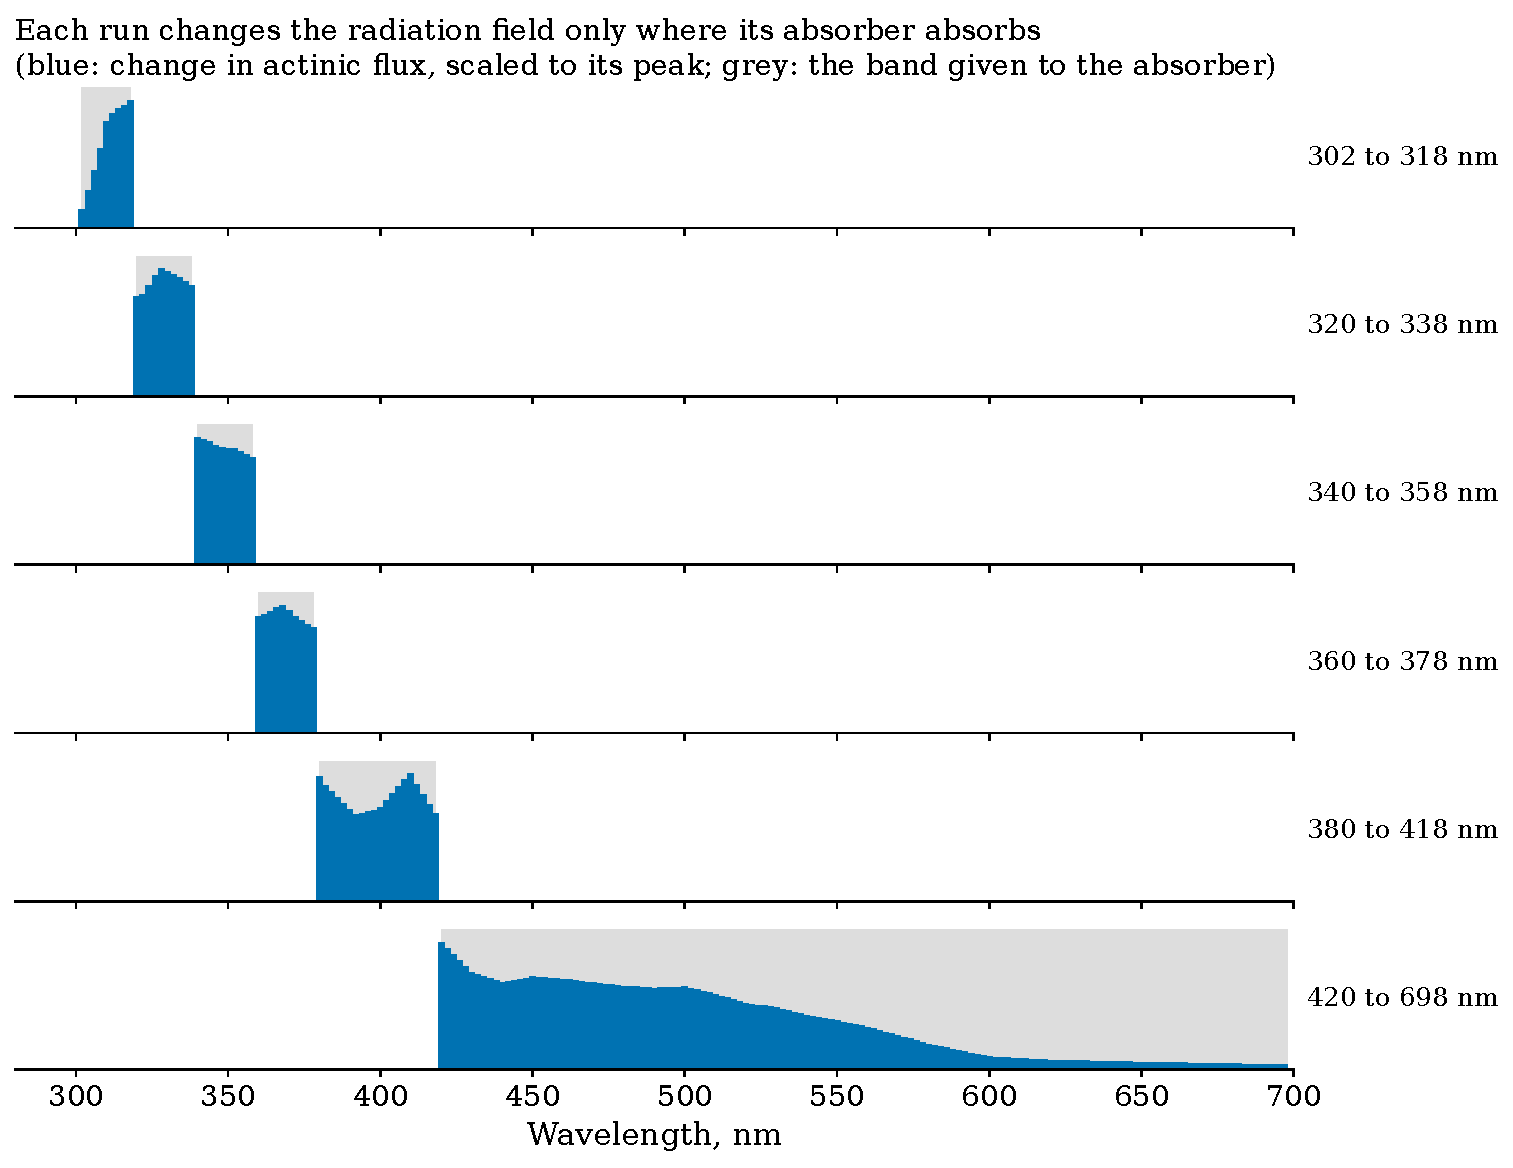
\includegraphics[width=\linewidth,height=0.76\textheight,keepaspectratio]{F07_E04_spectrally-local_ch5_s9.pdf}
    \end{column}
    \begin{column}{0.47\textwidth}
      \vskip4mm
      \finding{Each run limited to one window changes sunlight only in that window.}
      \small
      \renewcommand{\arraystretch}{1.25}
      \begin{tabular}{@{}lcr@{}}
        \toprule
        Molecule & Main window, nm & Share\\
        \midrule
        S\sub{2}O & 300 to 320 & 93.689\%\\
        SO\sub{3} & 300 to 320 & 80.754\%\\
        S\sub{3}  & 380 to 420 & 49.605\%\\
        S\sub{4}  & 420 to 620 & 100\%\\
        \bottomrule
      \end{tabular}
      \vskip4mm
      \normalsize
      \begin{itemize}
        \item Each molecule draws on its own part of the spectrum.
      \end{itemize}
    \end{column}
  \end{columns}
\end{frame}

% Slide 13. Report Sections 5.4 and 5.5, Figure F09 (F08 follows).
% Numbers: e6.R781.pct_in_band 99.128, .peak_z 71; R787 99.992 at 73; R593 peak 35.
\begin{frame}{Experiments 5 and 6: which reactions, which altitudes?}
  \begin{columns}[T,onlytextwidth]
    \begin{column}{0.48\textwidth}
      \centering
      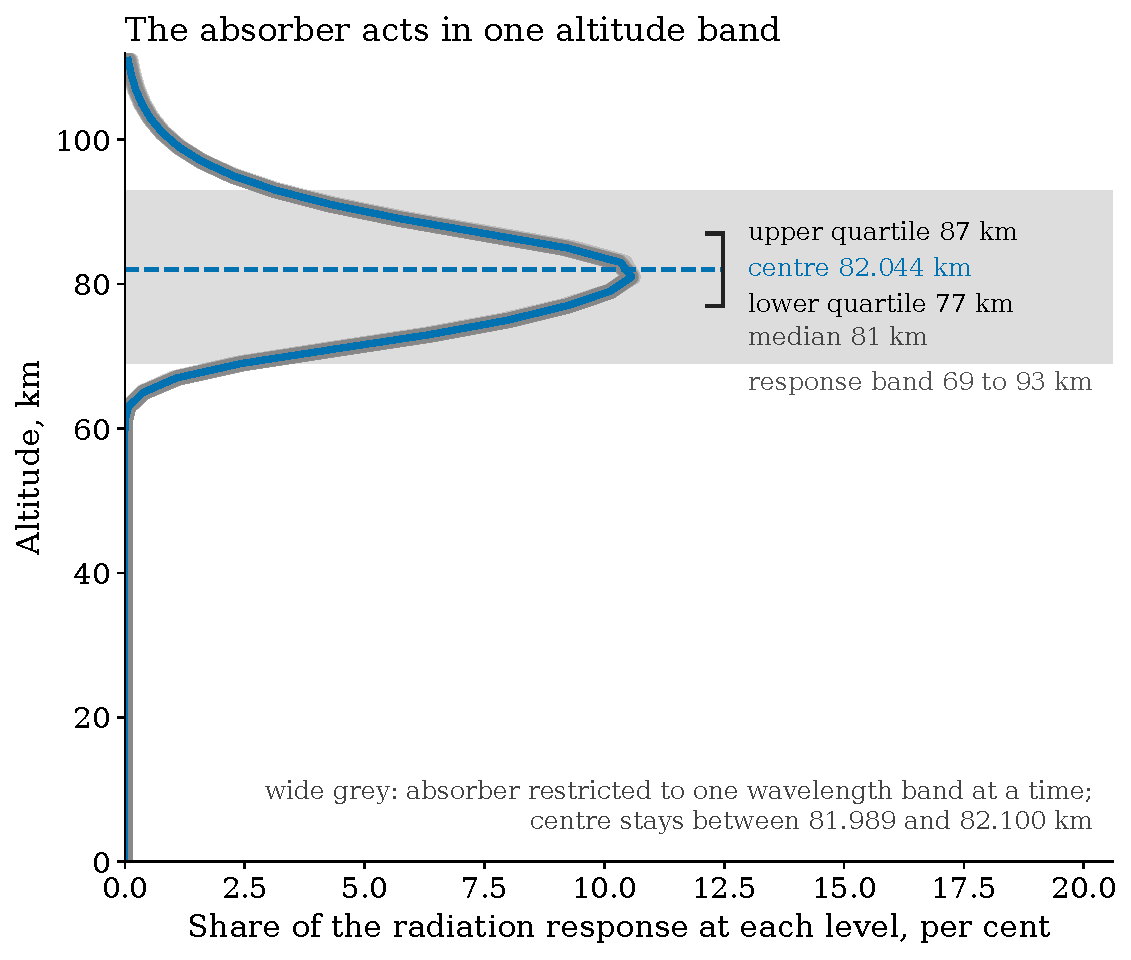
\includegraphics[width=\linewidth,height=0.76\textheight,keepaspectratio]{F09_E06_response-band_ch5_s10.pdf}
    \end{column}
    \begin{column}{0.49\textwidth}
      \vskip4mm
      \finding{The response sits in one band, 69 to 93 km, for every wavelength window tested.}
      \small
      \renewcommand{\arraystretch}{1.25}
      \begin{tabular}{@{}lcc@{}}
        \toprule
        Reaction & In the band & Peak\\
        \midrule
        SO\sub{2} photolysis & 99.128\% & 71 km\\
        SO\sub{3} photolysis & 99.992\% & 73 km\\
        COS + 2 SO\sub{3} & almost none & 35 km\\
        \bottomrule
      \end{tabular}
      \vskip4mm
      \normalsize
      \begin{itemize}\setlength{\itemsep}{1.5mm}
        \item Direct effects sit in the band; knock-on effects lie lower.
      \end{itemize}
    \end{column}
  \end{columns}
\end{frame}

% Slide 13b. Report Section 5.4, Figure F08.
% Numbers: e5.SO2.R593.maxdelta; e5.SO2.R663.frac_pct.
\begin{frame}{Experiment 5: the reactions behind the SO\sub{2} change}
  \finding{The largest absolute change is not the most affected reaction.}
  \centering
  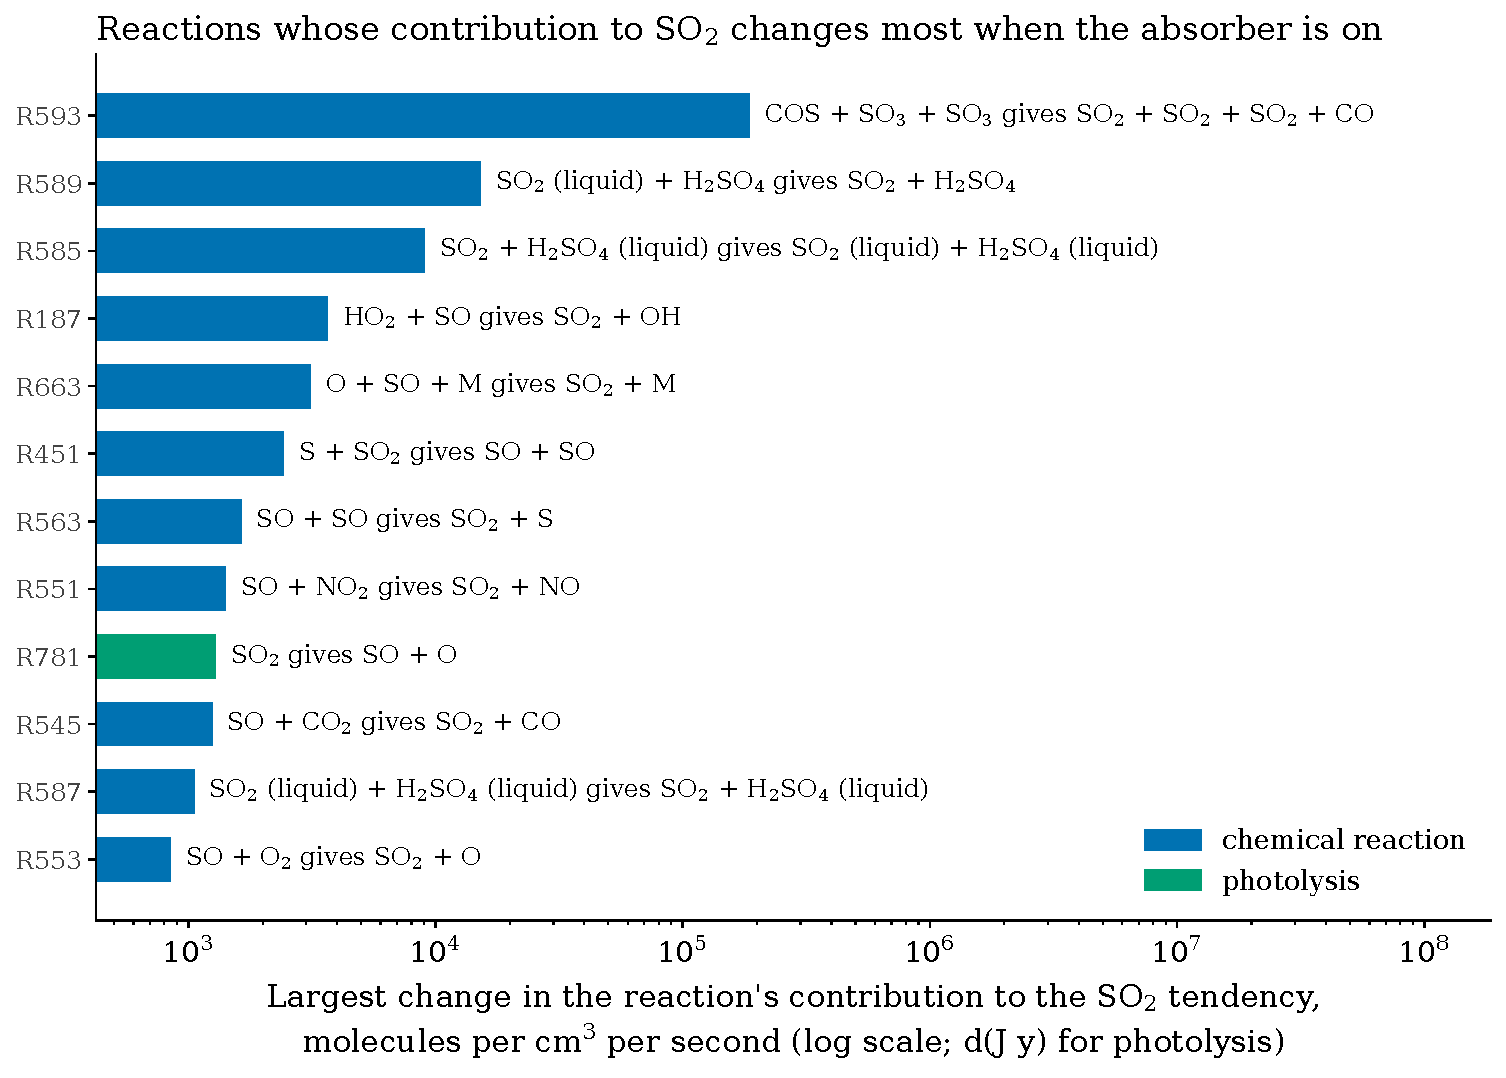
\includegraphics[width=\linewidth,height=0.68\textheight,keepaspectratio]{F08_E05_reaction-pathways_ch5_report.pdf}
\end{frame}

% Slide 14. Report Section 5.6, Figure F10.
% Numbers: e7.7a.centroid_shift 17.8439; e7.7b.centroid_shift -18.0000;
% e7a.L2pct 2.2498; e7b.L2pct 0.3067; e7.ratio_7A_over_7B 7.34; res.e7a.SO.inband 8.404;
% pnom.cloud 90.194.
\begin{frame}{Experiment 7: does placement matter?}
  \finding{Moved up, the same absorber has 7.34 times more effect than moved down.}
  \begin{columns}[T,onlytextwidth]
    \begin{column}{0.62\textwidth}
      \centering
      % The figure's own top line repeats the finding, so it is trimmed off here
      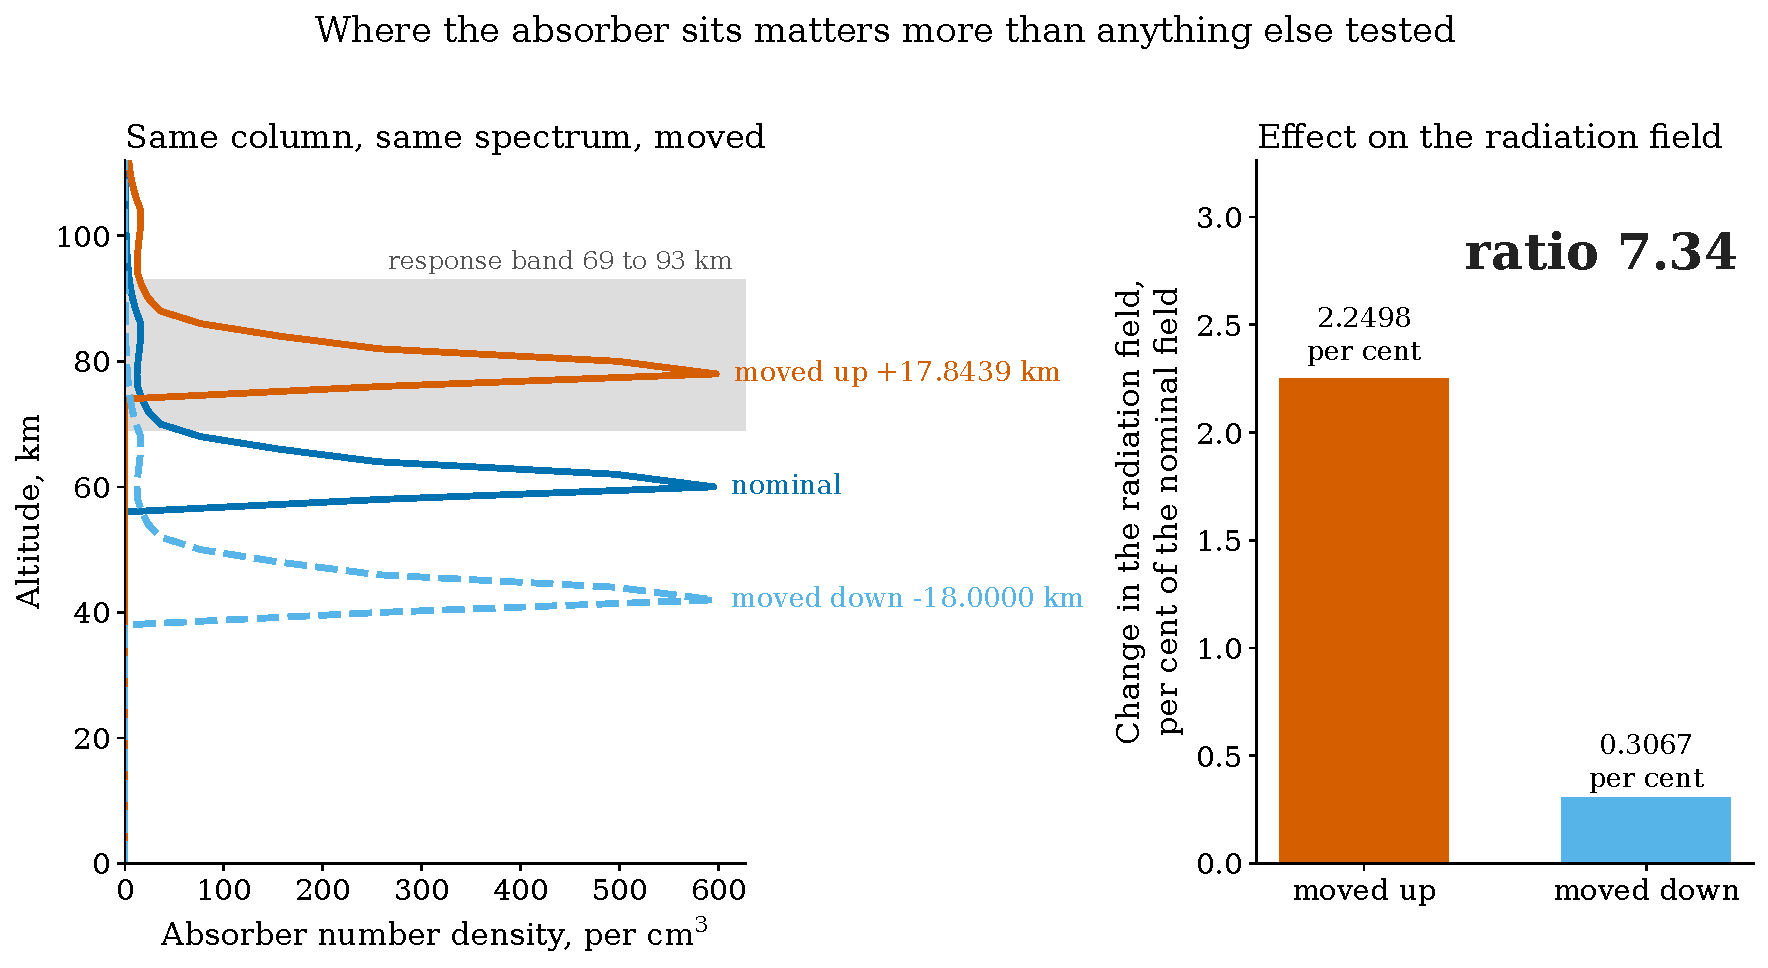
\includegraphics[trim=0 0 0 40,clip,width=\linewidth,height=0.70\textheight,keepaspectratio]{F10_E07_placement-first-order_ch5_s11.pdf}
    \end{column}
    \begin{column}{0.36\textwidth}
      \vskip4mm
      \small
      \renewcommand{\arraystretch}{1.25}
      \begin{tabular}{@{}lr@{}}
        \toprule
        Move & Change\\
        \midrule
        Up, $+$17.8439 km & 2.2498\%\\
        Down, $-$18.0000 km & 0.3067\%\\
        \midrule
        \textbf{Ratio} & \textbf{7.34}\\
        \bottomrule
      \end{tabular}
      \vskip3mm
      \begin{itemize}\setlength{\itemsep}{1.5mm}
        \item As supplied: 90.194\% at 58 to 69 km, below the band.
        \item Moved up, SO in the band: 8.404\%.
      \end{itemize}
    \end{column}
  \end{columns}
\end{frame}

% ===========================================================================
\section{Experiments 8 to 14}
% ===========================================================================

% Slide 15. Report Section 6.1, Figure F11.
% Numbers: tau.spec_change_pct 0.6461; e8a.L2pct, e8b.L2pct, e8c.L2pct and
% e7.ratio_7A_over_7B inside the figure.
\begin{frame}{Experiment 8: spectrum against placement}
  \finding{Same amount, same height, three spectra: shape matters, placement matters more.}
  \centering
  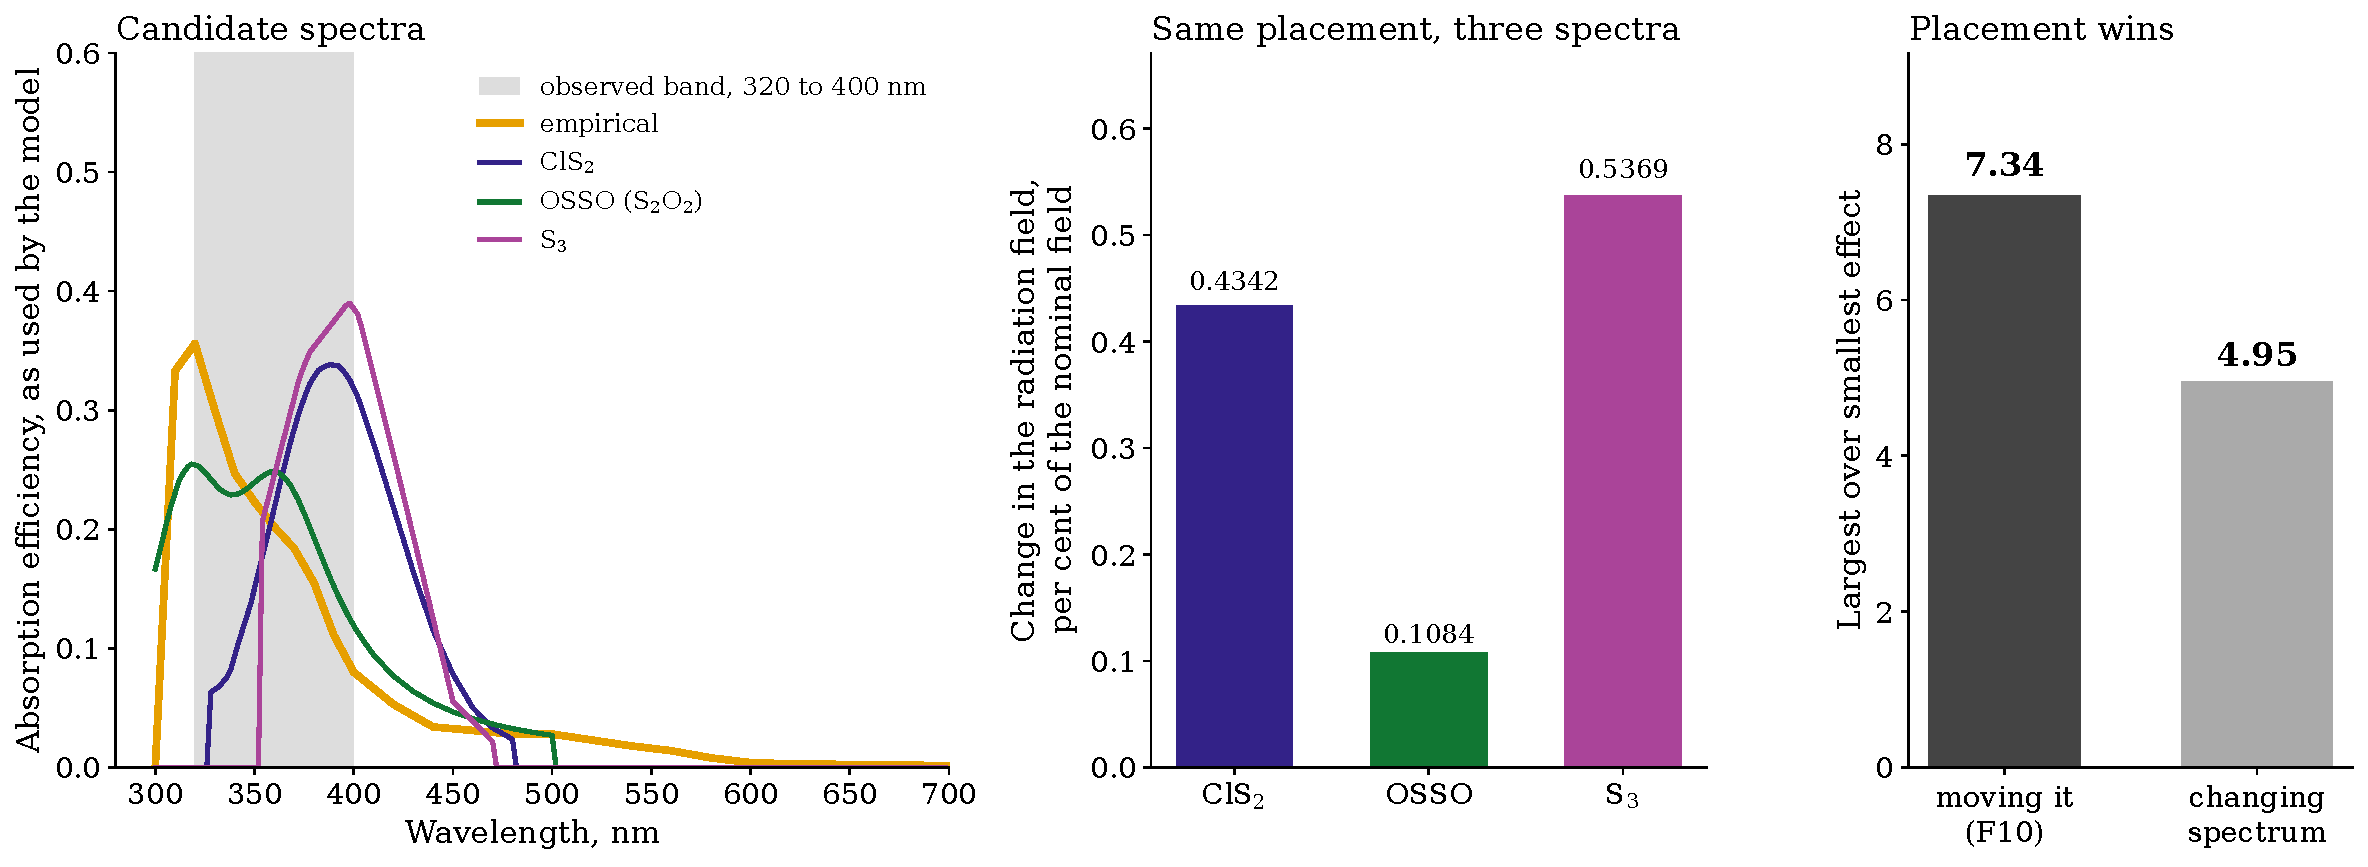
\includegraphics[width=\linewidth,height=0.60\textheight,keepaspectratio]{F11_E08_spectrum-vs-placement_ch6_s12.pdf}
  \par\vskip2mm
  \raggedright
  \begin{itemize}
    \item Spectra scaled to one total; optical depth above 69 km within 0.6461\%.
  \end{itemize}
\end{frame}

% Slide 16. Report Sections 6.1 to 6.3 (Experiment 10 folded in), Figure F12 (top line trimmed for the slide).
% Numbers: scr.ClS2.short 121.914; pnom.centroid 63.419; p9.centroid 13.656;
% pnom.inband 9.1940; p9.inband 0.0000; tau.reduction 2.0e8; id.l2_ratio_pct 0.001487.
\begin{frame}{Experiments 9 and 10: the chemistry places the candidate}
  \finding{Placed by its own chemistry, ClS\sub{2} falls out of the response band.}
  \begin{columns}[T,onlytextwidth]
    \begin{column}{0.58\textwidth}
      \centering
      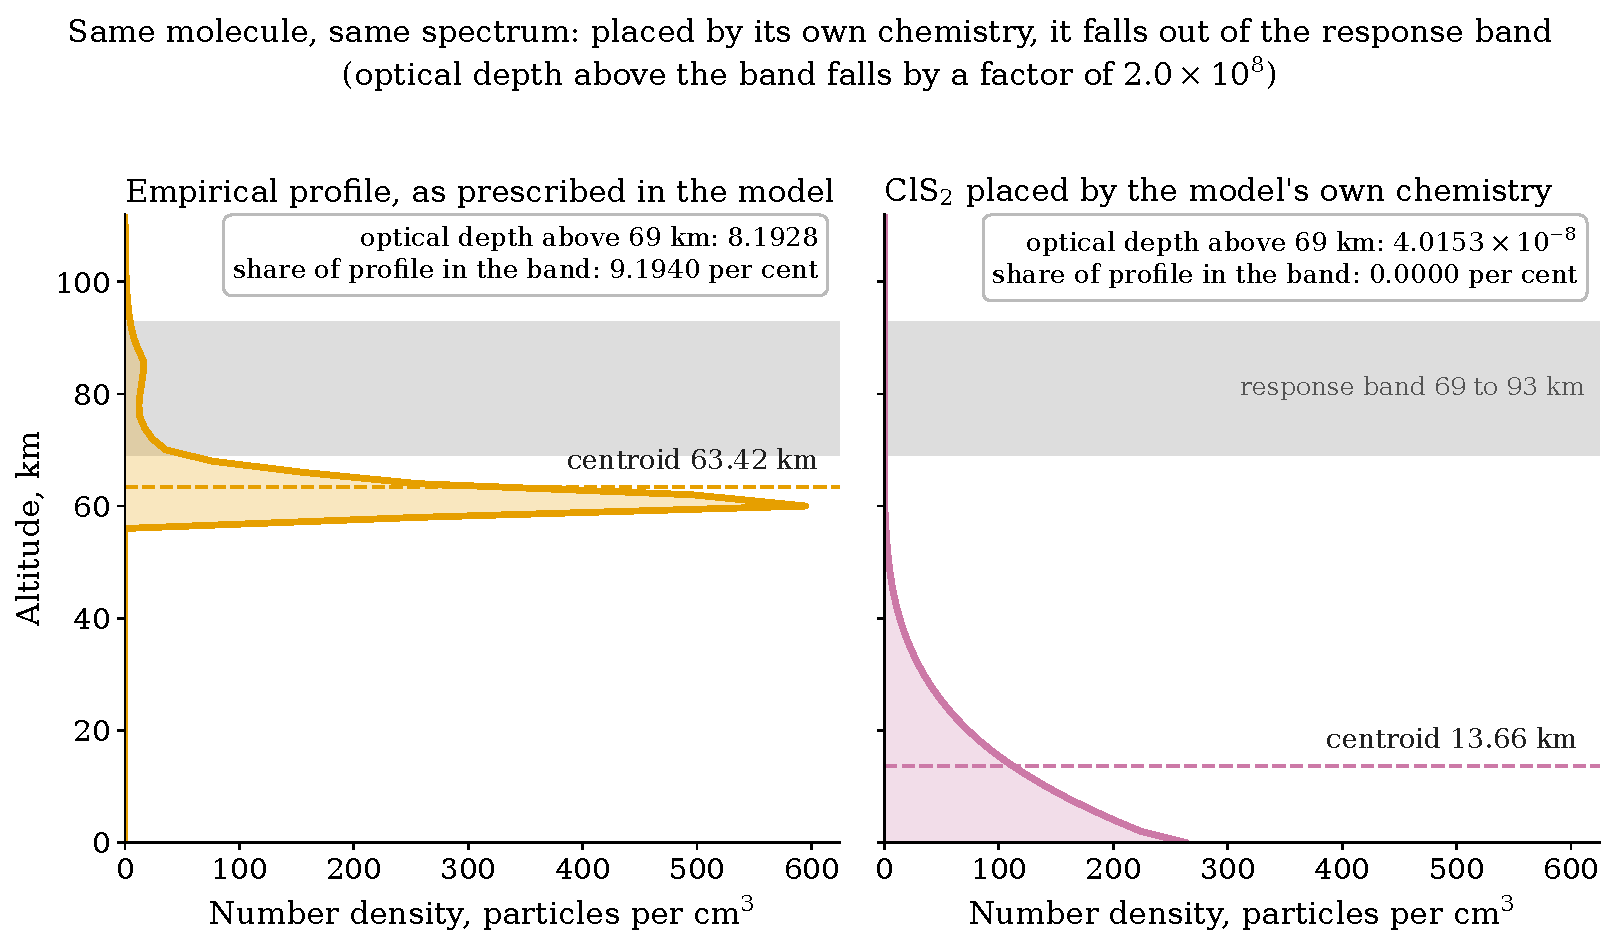
\includegraphics[width=\linewidth,height=0.70\textheight,keepaspectratio,trim=0 0 0 46,clip]{F12_E09_ClS2-self-placement_ch6_s13.pdf}
    \end{column}
    \begin{column}{0.39\textwidth}
      \small
      \renewcommand{\arraystretch}{1.25}
      \begin{tabular}{@{}lcc@{}}
        \toprule
        & Set & Chemistry\\
        \midrule
        Centre, km   & 63.419  & 13.656\\
        In band      & 9.1940\% & 0.0000\%\\
        \bottomrule
      \end{tabular}
      \vskip3mm
      \small
      \begin{itemize}\setlength{\itemsep}{0.8mm}
        \item Closest in amount, short by 121.914.
        \item Above 69 km: $2.0\times10^{8}$ times less optical depth.
        \item Same as no absorber, to 0.001487\%.
        \item Experiment 10, rerun with S\sub{3}: the same.
      \end{itemize}
    \end{column}
  \end{columns}
\end{frame}

% Slide 18. Report Section 6.4, Figure F14.
% Numbers: iso.SSCl2.val_pct 0.114; iso.SSCl2.val_nm 0.156; iso.ClSSCl.val_pct 0.079;
% iso.ClSSCl.val_nm 0.331; e11a.L2pct 0.19465; e11b.L2pct 0.30144;
% iso.SSCl2.short 4.266e5; iso.ClSSCl.short 6.668e6; share320400.11A 85.49.
\begin{frame}{Experiment 11: two computed isomer spectra}
  \finding{The authors' cross sections run as absorbers; neither isomer can be made in the amount needed.}
  \begin{columns}[T,onlytextwidth]
    \begin{column}{0.52\textwidth}
      \centering
      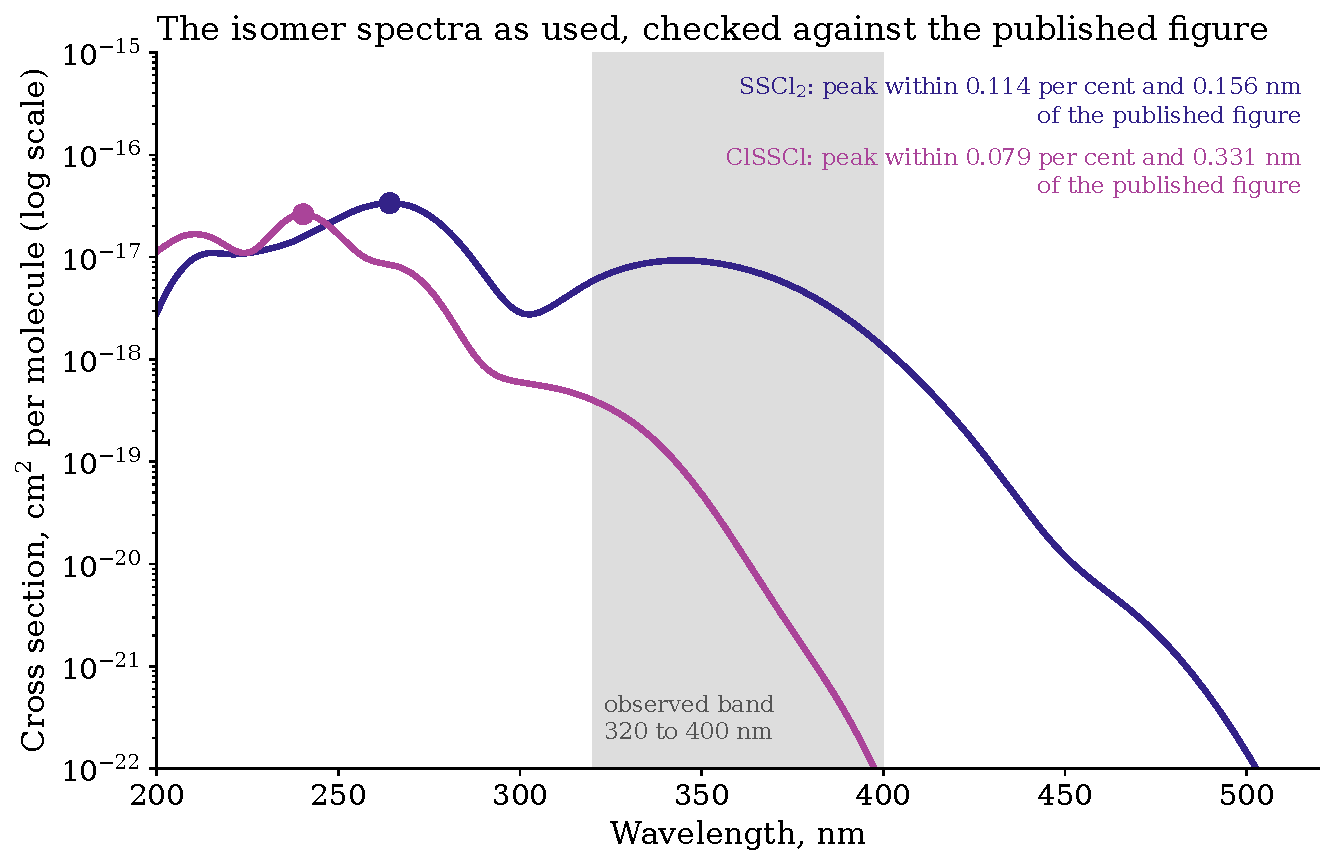
\includegraphics[width=\linewidth,height=0.64\textheight,keepaspectratio]{F14_E11_published-cross-sections_ch6_report.pdf}
    \end{column}
    \begin{column}{0.45\textwidth}
      \small
      \renewcommand{\arraystretch}{1.25}
      \begin{tabular}{@{}lcc@{}}
        \toprule
        & SSCl\sub{2} & ClSSCl\\
        \midrule
        Peak height         & 0.114\%  & 0.079\%\\
        Peak position       & 0.156 nm & 0.331 nm\\
        Field change        & 0.19465\% & 0.30144\%\\
        Short by            & $4.266\times10^{5}$ & $6.668\times10^{6}$\\
        \bottomrule
      \end{tabular}
      \vskip3mm
      \begin{itemize}
        \item SSCl\sub{2}: 85.49\% of its absorption at 320 to 400 nm, the most tested.
        \item ClSSCl peaks below 300 nm; the model sees its tail.
      \end{itemize}
    \end{column}
  \end{columns}
  \refline{Trabelsi and Francisco (2026)}
\end{frame}

% Slide 19. Report Sections 1.5 and 6.5, Figure F03.
% Numbers inside the figure: e12.n_screened 23; e12.gate.n_placement 16; two pass
% placement and spectrum; e12.gate.n_all 0; e12.gate.emp_inband_pct 11.92;
% e12.S2O2.short.360 2.5e5; e12.HOCl.short.360 1.0e7.
\begin{frame}{Experiment 12: all three tests on every species}
  \finding{Twenty-three species screened; none passes all three tests.}
  \centering
  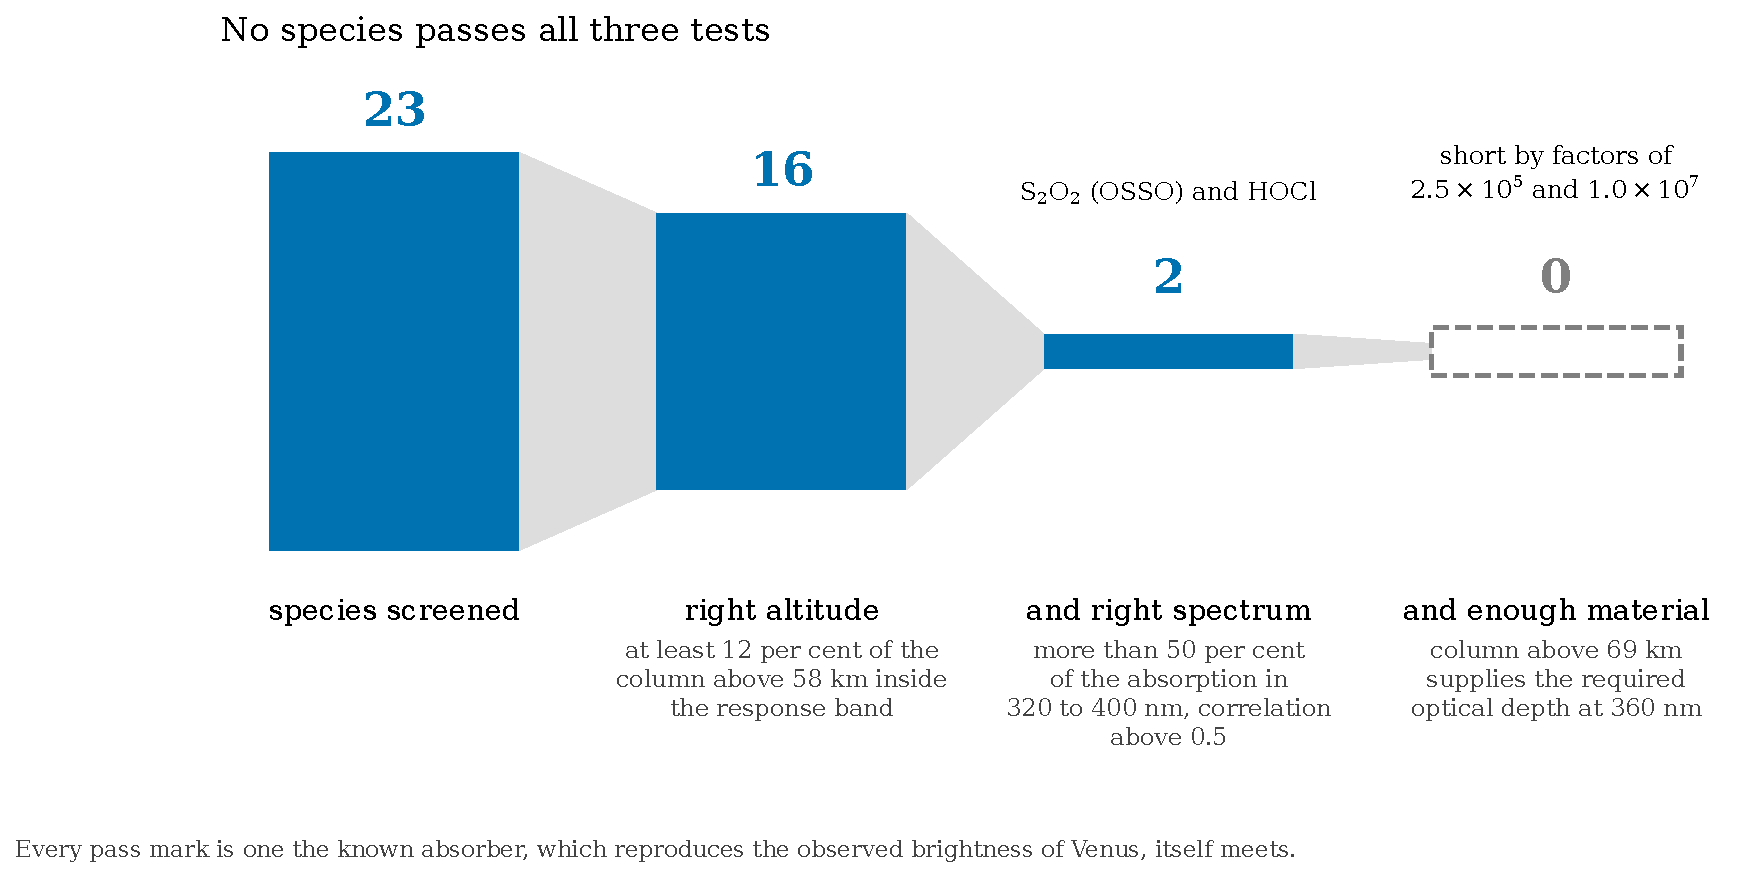
\includegraphics[width=\linewidth,height=0.66\textheight,keepaspectratio]{F03_CTX_three-gates_ch1_backup.pdf}
\end{frame}

% Slide 20. Report Section 6.5, Figure F15.
% Numbers inside the figure: e12.X.short.360, e12.X.frac_in_band_pct, e12.X.corr.
\begin{frame}{Experiment 12: the three tests disagree}
  \finding{Amount is a gate; on the other two tests each picks a different best species.}
  \centering
  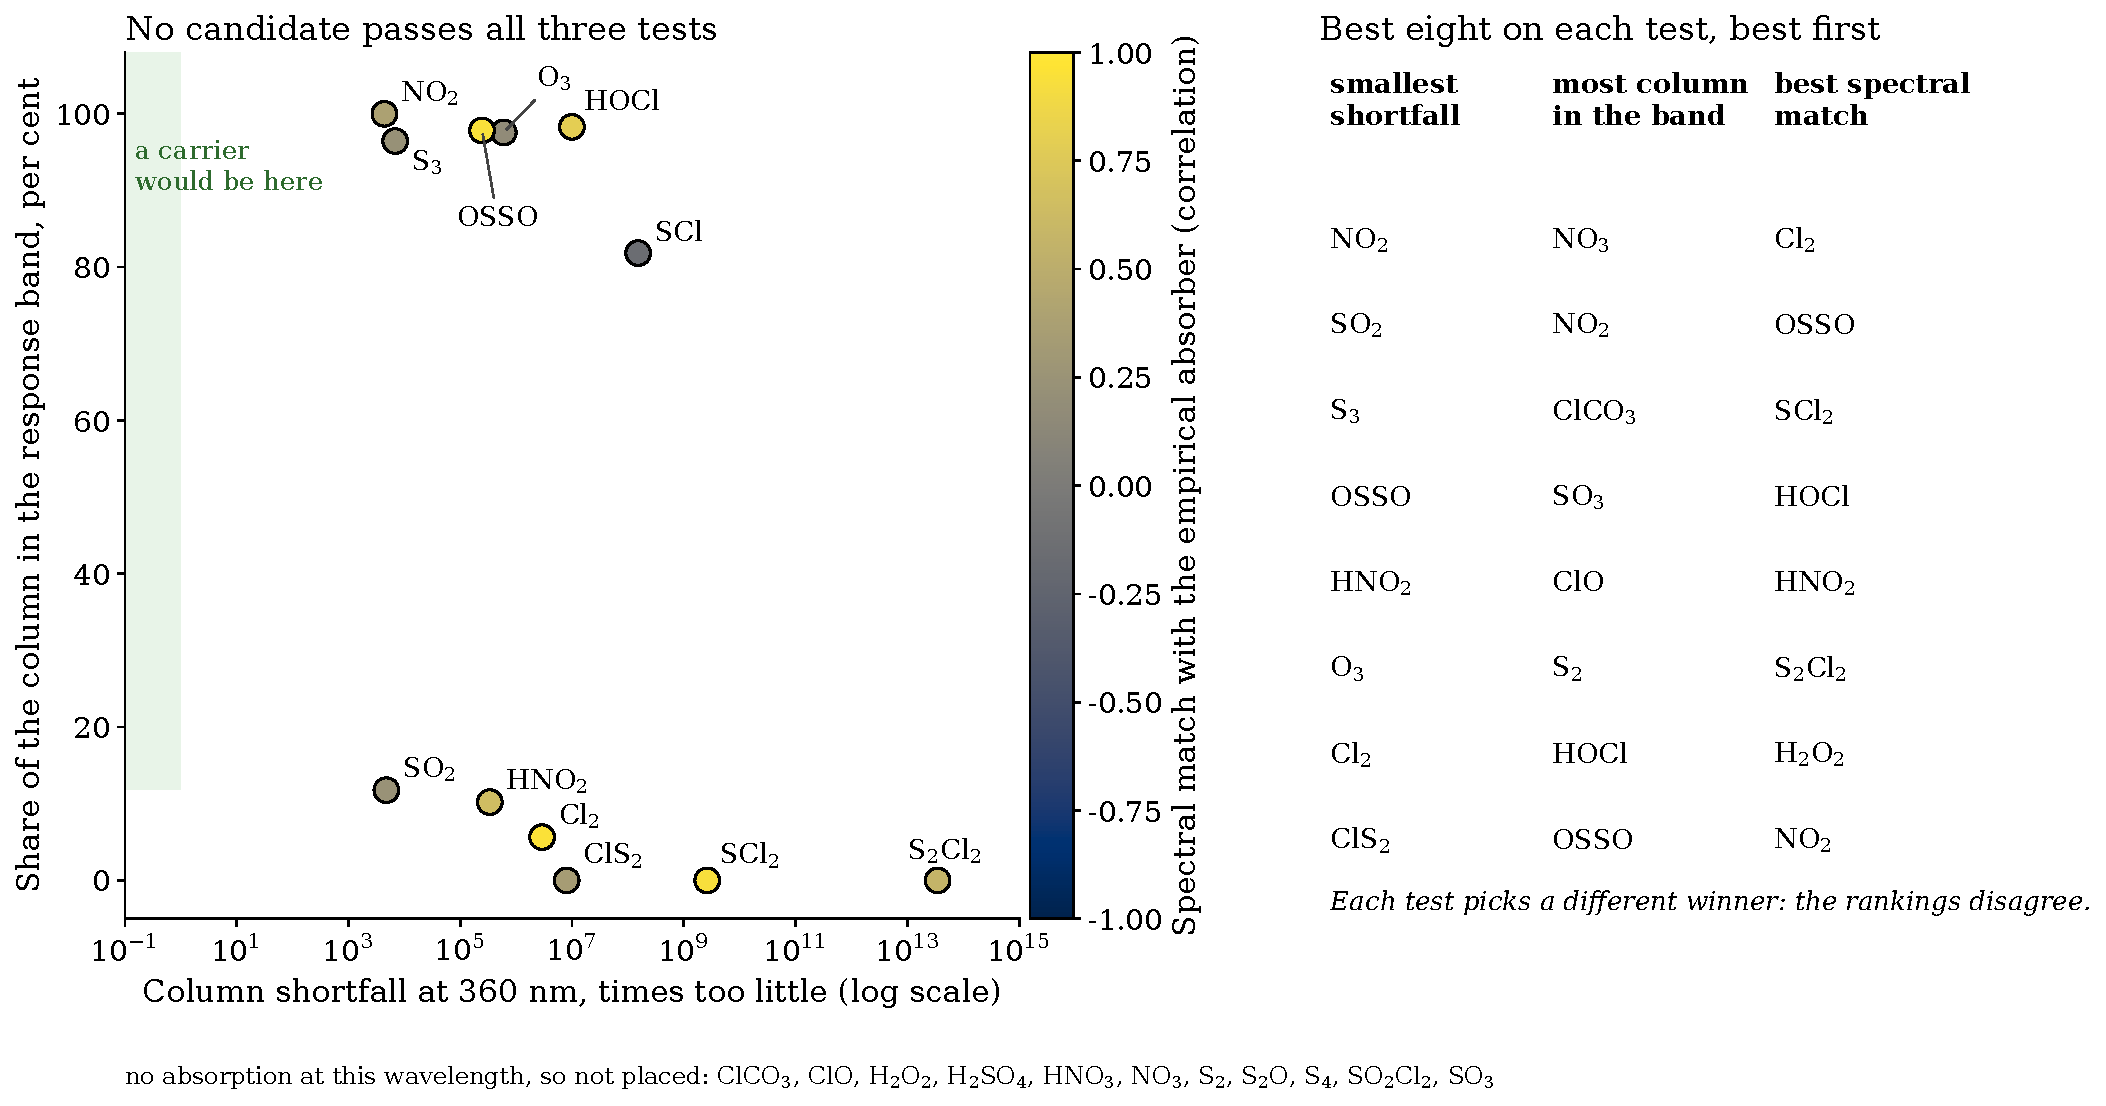
\includegraphics[width=\linewidth,height=0.70\textheight,keepaspectratio]{F15_E12_three-axis-screen_ch6_s14.pdf}
\end{frame}

% Slide 21. Report Section 6.6, Figure F16.
% Numbers: e13.A_required 1278; figure values e13.*.
\begin{frame}{Experiment 13: iron and sulfur minerals}
  \finding{Even a droplet made wholly of either mineral could not absorb enough at 375 nm.}
  \centering
  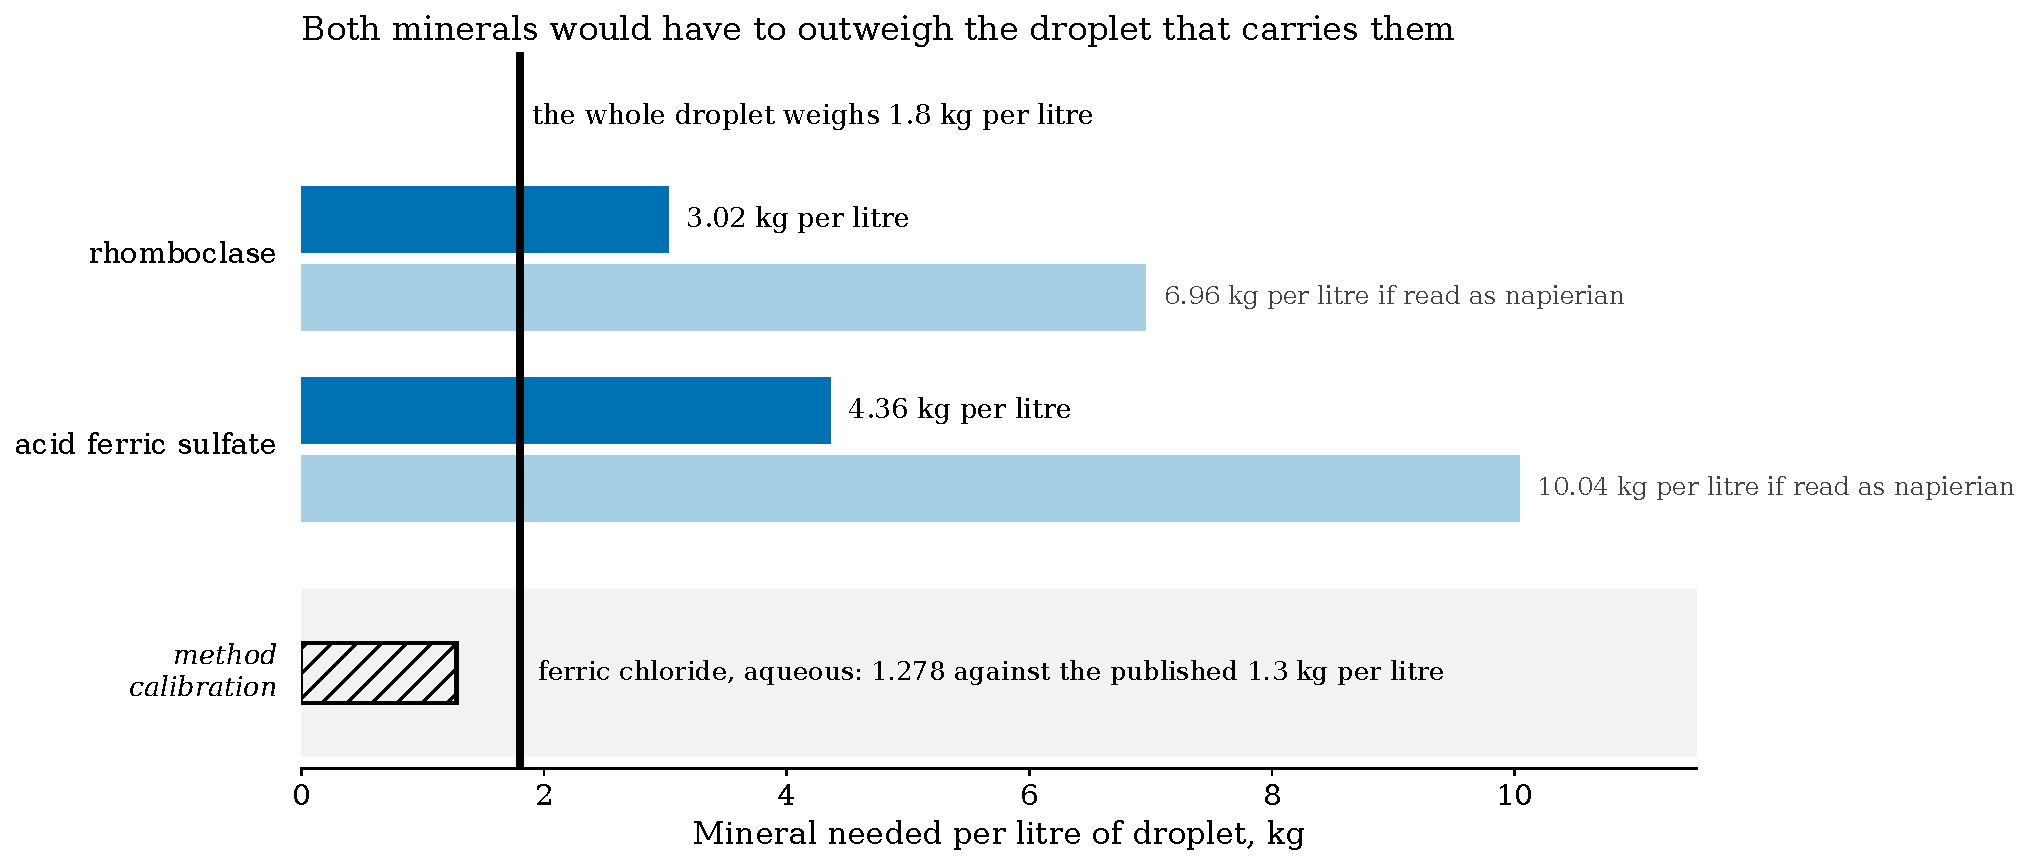
\includegraphics[width=\linewidth,height=0.55\textheight,keepaspectratio]{F16_E13_minerals-cannot-reach_ch6_s15.pdf}
  \par\vskip1mm
  \raggedright
  \begin{itemize}
    \item Requirement: 1278 per cm at 375 nm; coefficients as measured by Jiang et al.
  \end{itemize}
  \refline{Jiang et al.\ (2024); Spacek et al.\ (2026)}
\end{frame}

% Slide 22. Report Sections 6.7 and 6.8, Figure F17 (top line trimmed for the slide).
% Numbers: e14.aqueous_pct_of_droplet 71.0; e14.ClA.pct_of_droplet 2.82;
% e14.ClE.pct_of_droplet 17.05; e14.factor_to_fit_after 2.6 inside the figure.
\begin{frame}{Experiment 14: ferric chloride in acid}
  \finding{Measured in hydrochloric acid, ferric chloride needs 2.82\% to 17.05\% of the droplet, not 71.0\%.}
  \centering
  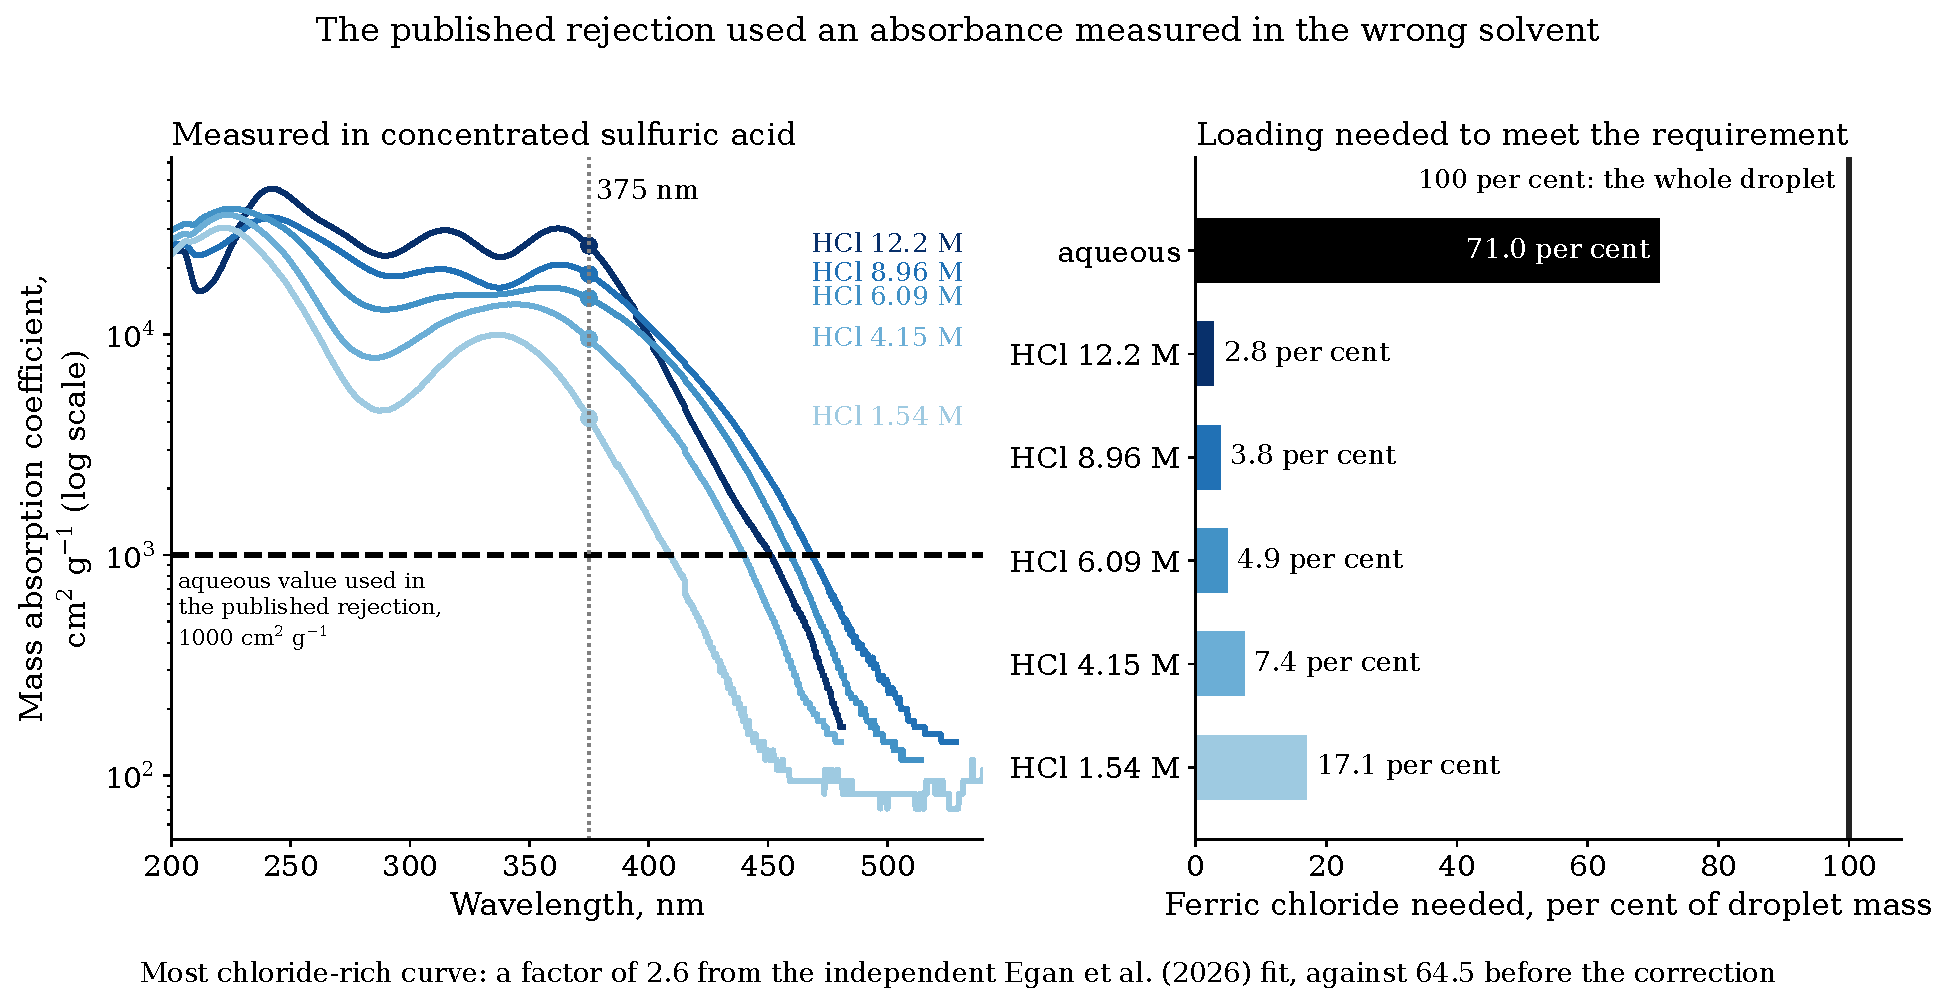
\includegraphics[width=\linewidth,height=0.55\textheight,keepaspectratio,trim=0 0 0 30,clip]{F17_E14_ferric-chloride-correction_ch6_s16.pdf}
  \par\vskip1mm
  \raggedright
  \begin{itemize}
    \item The rejection rested on water; altitude is still untested.
  \end{itemize}
  \refline{Spacek et al.\ (2026); Egan, James and Plane (2025); Egan et al.\ (2026)}
\end{frame}

% ===========================================================================
\section{Findings and Verification}
% ===========================================================================

% Slide 23. Report Section 7.1.
% Numbers: e10.fielddiff_pct 0.0017; res.e10.SO.inband 2.5278; e6.interval.90.lo, .hi;
% e7.ratio_7A_over_7B 7.34; e8c.L2pct over e8b.L2pct 4.95.
\begin{frame}{What Phase 1 establishes}
  \vskip2mm
  \centering
  \small
  \renewcommand{\arraystretch}{1.35}
  \begin{tabular}{@{}L{0.62\textwidth}l@{}}
    \toprule
    \textbf{Result} & \textbf{Basis}\\
    \midrule
    The absorber acts within one band, 69 to 93 km & Measured\\
    Placement beats spectrum: 7.34 against 4.95 & Measured\\
    Placed by its own chemistry, ClS\sub{2} equals no absorber & Measured\\
    No species in the model passes all three tests & Calculated, model output\\
    Minerals fall short; the ferric chloride rejection is reopened & Calculated, published data\\
    Chemical responses mostly below the floor & Bounded\\
    \bottomrule
  \end{tabular}
  \vskip5mm
  \raggedright
  \begin{itemize}
    \item Measured: radiative, reproducible to 0.0017\% of the change.
    \item Bounded: abundances, reproducible only to 2.5278\%.
  \end{itemize}
\end{frame}

% Slide 24. Report Section 7.2. Numbers: e12.n_screened 23; e12.n_tracked 62.
\begin{frame}{The limits}
  \vskip2mm
  \centering
  \small
  \renewcommand{\arraystretch}{1.35}
  \begin{tabular}{@{}L{0.36\textwidth}L{0.56\textwidth}@{}}
    \toprule
    \textbf{Limit} & \textbf{What it means}\\
    \midrule
    One column, one sun angle & No latitude, no local time, steady states only\\
    Weak vertical mixing      & Placement tested at one mixing strength\\
    Simplified droplets       & Fitted cross sections; full droplet calculation off\\
    Empirical reference       & Spectral rankings measure resemblance to a fit\\
    Only what the network holds & 23 of 62 species could be screened\\
    Floor from one pair of runs & A lower bound on the numerical scatter\\
    \bottomrule
  \end{tabular}
  \vskip5mm
  \raggedright
  \finding{Every run shares these limits, so comparisons stand; Phase 2 takes up the first two.}
\end{frame}

% Slide 25. Report Sections 8.1 to 8.3. Numbers: registry size 10830;
% 407 checked numbers in Chapters 1 to 10 and 129 in the figures (Section 8.2).
\begin{frame}{Verification: no number typed by hand}
  \finding{Every number is recomputed from the saved output and checked on the page.}
  \vskip5mm
  \centering
  % One size for every box: 22 mm wide, 14 mm tall
  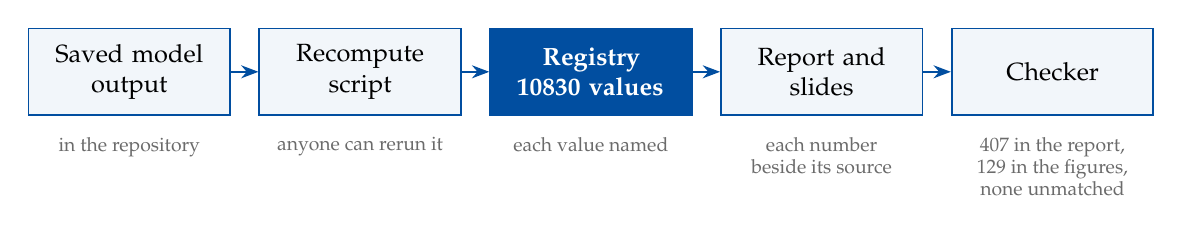
\begin{tikzpicture}[node distance=3.5mm,
      every node/.append style={minimum height=14mm}]
    \node[box=22mm] (a) {Saved model\\output};
    \node[box=22mm, right=of a] (b) {Recompute\\script};
    \node[keybox=22mm, right=of b] (c) {Registry\\10830 values};
    \node[box=22mm, right=of c] (d) {Report and\\slides};
    \node[box=22mm, right=of d] (e) {Checker};
    \draw[flow] (a) -- (b); \draw[flow] (b) -- (c);
    \draw[flow] (c) -- (d); \draw[flow] (d) -- (e);
    \node[note, below=1.5mm of a, minimum height=0pt] {in the repository};
    \node[note, below=1.5mm of b, minimum height=0pt] {anyone can rerun it};
    \node[note, below=1.5mm of c, minimum height=0pt] {each value named};
    \node[note, below=1.5mm of d, minimum height=0pt] {each number\\beside its source};
    \node[note, below=1.5mm of e, minimum height=0pt] {407 in the report,\\129 in the figures,\\none unmatched};
  \end{tikzpicture}
  \vskip6mm
  \raggedright
  \begin{itemize}
    \item The checker proves a number is in the registry, not that it is the right one.
    \item So every number was also checked by hand against its own entry.
  \end{itemize}
\end{frame}

% ===========================================================================
\section{Future work}
% ===========================================================================

% Slide 27. Report Chapter 9: Section 9.1, Figure F19, and Section 9.4.
% Numbers: p2.gap.Bkzz.t_days 552; figure values p2.*.
\begin{frame}{Future work}
  \finding{Phase 2: can realistic transport carry a candidate into the response band?}
  \begin{columns}[T,onlytextwidth]
    \begin{column}{0.57\textwidth}
      \centering
      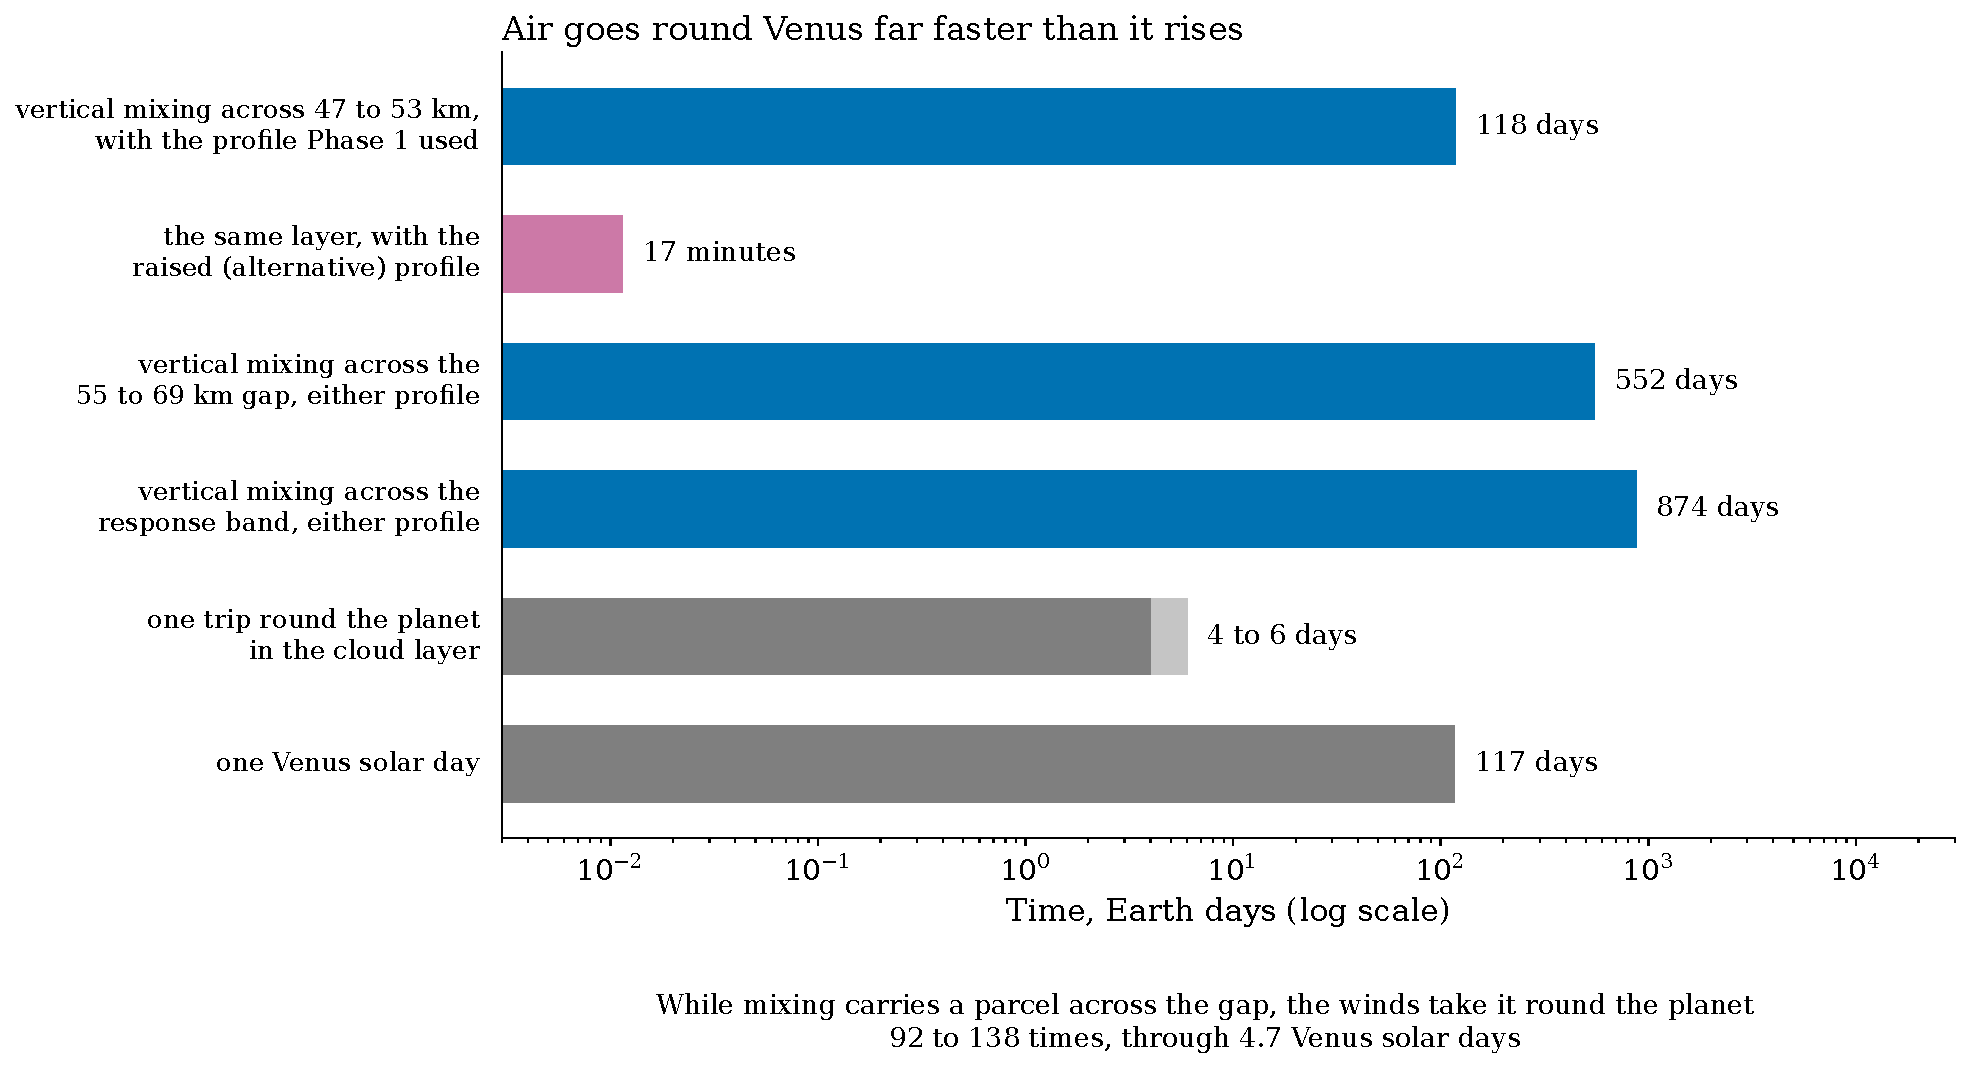
\includegraphics[width=\linewidth,height=0.52\textheight,keepaspectratio]{F19_P2_transport-timescales_ch9_s19.pdf}
      \par\vskip1mm
      \raggedright
      {\small Mixing needs 552 days to cross the 55 to 69 km gap; the winds circle Venus in 4 to 6.\par}
    \end{column}
    \begin{column}{0.40\textwidth}
      \colhead{Six work packages}
      \centering
      % One size for every box: 24 mm wide, 9 mm tall
      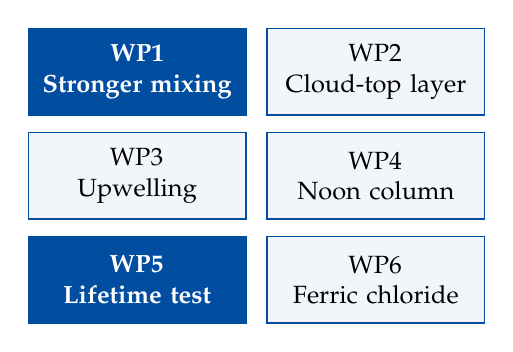
\begin{tikzpicture}[node distance=2mm and 2.5mm,
          every node/.append style={minimum height=9mm, font=\small}]
        \node[keybox=24mm] (w1) {WP1\\Stronger mixing};
        \node[box=24mm, right=of w1] (w2) {WP2\\Cloud-top layer};
        \node[box=24mm, below=of w1] (w3) {WP3\\Upwelling};
        \node[box=24mm, below=of w2] (w4) {WP4\\Noon column};
        \node[keybox=24mm, below=of w3] (w5) {WP5\\Lifetime test};
        \node[box=24mm, below=of w4] (w6) {WP6\\Ferric chloride};
      \end{tikzpicture}
      \par\vskip2mm
      \raggedright
      {\small WP1 and WP5 first, ferric chloride last.\par}
    \end{column}
  \end{columns}
  \refline{Limaye et al.\ (2018); Bertaux et al.\ (2016)}
\end{frame}

% ===========================================================================
\section{Summary}
% ===========================================================================

% Slide 31. Report Section 10.1. Band: e6.interval.90.lo and .hi.
\begin{frame}{Summary}
  \vskip3mm
  \begin{itemize}\setlength{\itemsep}{4mm}
    \item Switched on, the absorber acts in one band: 69 to 93 km.
    \item Where an absorber sits matters more than its spectrum.
    \item The chemistry, not the modeller, decides where a candidate sits.
    \item No species in the model passes all three tests.
    \item Minerals fall short; ferric chloride is reopened, its altitude untested.
    \item Every number traces back to the saved output.
  \end{itemize}
  \vskip4mm
  \finding{Next: can realistic mixing carry a candidate into the band?}
\end{frame}

% ===========================================================================
\section{References and Sources}
% ===========================================================================

% Taken from report/references.tex; long author lists shortened to the first author.
\begin{frame}{References}
  \scriptsize
  \renewcommand{\arraystretch}{1.0}
  \setlength{\parskip}{1.2mm}
  \raggedright
  Bertaux, J.-L., et al.\ (2016). Influence of Venus topography on the zonal wind and UV albedo at cloud top level: the role of stationary gravity waves. \emph{J.\ Geophys.\ Res.\ Planets} 121, 1087 to 1101.\par
  Bierson, C.\ J., and Zhang, X.\ (2020). Chemical cycling in the Venusian atmosphere: a full photochemical model from the surface to 110 km. \emph{J.\ Geophys.\ Res.\ Planets} 125, e2019JE006159.\par
  Dai, L., Shao, W., Gu, H., and Sheng, Z.\ (2023). Determination of the eddy diffusion in the Venusian clouds from VeRa sulfuric acid observations. \emph{Astron.\ Astrophys.} 679, A155.\par
  Dai, L., Shao, W., and Sheng, Z.\ (2024). An investigation into Venusian atmospheric chemistry based on an open-access photochemistry-transport model at 0 to 112 km. \emph{Astron.\ Astrophys.} 689, A55.\par
  Dai, L., et al.\ (2025). Venus cloud research: progress and perspectives. \emph{Space Sci.\ Rev.} 221, 51.\par
  Egan, J.\ V., et al.\ (2025). Is OSSO a significant contributor to the unknown UV absorber in Venus' atmosphere? \emph{Geophys.\ Res.\ Lett.} 52, e2024GL113090.\par
  Egan, J.\ V., James, A.\ D., and Plane, J.\ M.\ C.\ (2025). Laboratory measurements of ferric chloride (FeCl\sub{3}) under Venusian conditions. \emph{ACS Earth Space Chem.}\par
  Egan, J.\ V., et al.\ (2026). Ferric chloride: the Venusian unknown UV absorber? Preprint, ESS Open Archive, not peer reviewed.\par
  Jiang, C.\ Z., et al.\ (2024). Iron-sulfur chemistry can explain the ultraviolet absorber in the clouds of Venus. \emph{Sci.\ Adv.} 10, eadg8826.\par
\end{frame}

\begin{frame}{References}
  \scriptsize
  \setlength{\parskip}{1.2mm}
  \raggedright
  Lef\`evre, M., Marcq, E., and Lef\`evre, F.\ (2022). The impact of turbulent vertical mixing in the Venus clouds on chemical tracers. \emph{Icarus} 386, 115148.\par
  Lef\`evre, M., et al.\ (2024). Impact of the turbulent vertical mixing on chemical and cloud species in the Venus cloud layer. \emph{Geophys.\ Res.\ Lett.} 51, e2024GL108771.\par
  Limaye, S.\ S., et al.\ (2018). Venus' spectral signatures and the potential for life in the clouds. \emph{Astrobiology} 18(9), 1181 to 1198.\par
  P\'erez-Hoyos, S., et al.\ (2018). Venus upper clouds and the UV absorber from MESSENGER/MASCS observations. \emph{J.\ Geophys.\ Res.\ Planets} 123, 145 to 162.\par
  Rimmer, P.\ B., et al.\ (2021). Hydroxide salts in the clouds of Venus: their effect on the sulfur cycle and cloud droplet pH. \emph{Planet.\ Sci.\ J.} 2, 133.\par
  Spacek, J., Rimmer, P.\ B., Petkowski, J.\ J., and Lee, Y.\ J.\ (2026). A model of UV-blue absorbance in bulk liquid of Venusian cloud aerosols is consistent with efficient organic absorbers at high concentrations. \emph{Astrobiology} 26(9), 727 to 739.\par
  Titov, D.\ V., et al.\ (2008). Atmospheric structure and dynamics as the cause of ultraviolet markings in the clouds of Venus. \emph{Nature} 456, 620 to 623.\par
  Trabelsi, T., and Francisco, J.\ S.\ (2026). Chlorine-sulfur isomers as parents of ClS\sub{2} and SCl\sub{2} on Venus: spectroscopy and photochemistry of ClSSCl, SSCl\sub{2}, and (ClS)\sub{2}. \emph{J.\ Chem.\ Phys.} 164, 084302.\par
\end{frame}

% Every result number on the slides, its registry entry and its report section.
\begin{frame}{Numbers and their sources (1 of 4)}
  \centering
  \scriptsize
  \renewcommand{\arraystretch}{1.12}
  \setlength{\tabcolsep}{4pt}
  \begin{tabular}{@{}rL{0.28\textwidth}L{0.40\textwidth}c@{}}
    \toprule
    \textbf{Number} & \textbf{What it is} & \textbf{Registry entry} & \textbf{Report}\\
    \midrule
    1.095 & Optical depth needed at 320 nm & \texttt{const.tau\_req} & 3.6\\
    2.2498\% & Field change, absorber moved up & \texttt{e7a.L2pct} & 5.6\\
    0.3067\% & Field change, absorber moved down & \texttt{e7b.L2pct} & 5.6\\
    7.34 & Ratio of the two moves & \texttt{e7.ratio\_7A\_over\_7B} & 5.6\\
    69 to 93 km & Response band, 90 per cent share & \texttt{e6.interval.90.lo, .hi} & 4.5\\
    90.194\% & Absorber at 58 to 69 km, as supplied & \texttt{pnom.cloud} & 4.5\\
    0.0017\% & Radiation floor, share of the change & \texttt{e10.fielddiff\_pct} & 6.3\\
    0.7384, 2.5278\% & SO in the band, Experiments 9 and 10 & \texttt{res.e9.SO.inband, res.e10.SO.inband} & 6.3\\
    0.013553\% & Experiment 1, mean change & \texttt{e1.aflux.meanrel} & 5.1\\
    \bottomrule
  \end{tabular}
  \par\vskip2mm{\scriptsize\color{softgrey}Set-up values come from the model files (report Table 3.1); literature values are cited on their slides.\par}
\end{frame}

\begin{frame}{Numbers and their sources (2 of 4)}
  \centering
  \scriptsize
  \renewcommand{\arraystretch}{1.12}
  \setlength{\tabcolsep}{4pt}
  \begin{tabular}{@{}rL{0.28\textwidth}L{0.40\textwidth}c@{}}
    \toprule
    \textbf{Number} & \textbf{What it is} & \textbf{Registry entry} & \textbf{Report}\\
    \midrule
    87.404\% & Largest change in sunlight & \texttt{e3fp.bnd.A1.aflux.max\_pct} & 5.1\\
    0.2243, 1.7399\% & Largest SO\sub{2} and SO changes & \texttt{e2.SO2.maxrel, e2.SO.maxrel} & 5.1\\
    1.00002, 1.00208 & Proportionality, optical depth and flux & \texttt{e3.lin.tau.inband.median, e3.lin.aflux.inband.median} & 5.2\\
    1.010795, 0.979304 & Proportionality at half and twice the amount & \texttt{e3fp.aflux.ratio.A0p5, .A2p0} & 5.2\\
    93.689, 80.754, 49.605, 100\% & Main-window shares, S\sub{2}O, SO\sub{3}, S\sub{3}, S\sub{4} & \texttt{e4a.<species>\_1.<window>.pct} & 5.3\\
    99.128\%, 71 km & SO\sub{2} photolysis in the band, its peak & \texttt{e6.R781.pct\_in\_band, .peak\_z} & 5.5\\
    99.992\%, 73 km & SO\sub{3} photolysis in the band, its peak & \texttt{e6.R787.pct\_in\_band, .peak\_z} & 5.5\\
    35 km & Peak of the knock-on reaction & \texttt{e6.R593.peak\_z} & 5.5\\
    17.8439, 18.0000 km & Centre moved up, moved down & \texttt{e7.7a.centroid\_shift, e7.7b.centroid\_shift} & 5.6\\
    8.404\% & SO in the band, absorber moved up & \texttt{res.e7a.SO.inband} & 5.6\\
    0.6461\% & Optical depth difference between spectra & \texttt{tau.spec\_change\_pct} & 6.1\\
    4.95 & Largest over smallest spectral effect & \texttt{e8c.L2pct over e8b.L2pct} & 6.1\\
    \bottomrule
  \end{tabular}
\end{frame}

\begin{frame}{Numbers and their sources (3 of 4)}
  \centering
  \scriptsize
  \renewcommand{\arraystretch}{1.12}
  \setlength{\tabcolsep}{4pt}
  \begin{tabular}{@{}rL{0.28\textwidth}L{0.40\textwidth}c@{}}
    \toprule
    \textbf{Number} & \textbf{What it is} & \textbf{Registry entry} & \textbf{Report}\\
    \midrule
    121.914 & ClS\sub{2} shortfall, Experiment 8 & \texttt{scr.ClS2.short} & 6.1\\
    63.419, 13.656 km & Centre, set and by chemistry & \texttt{pnom.centroid, p9.centroid} & 6.2\\
    9.1940, 0.0000\% & Share in the band, set and by chemistry & \texttt{pnom.inband, p9.inband} & 6.2\\
    $2.0\times10^{8}$ & Fall in optical depth above 69 km & \texttt{tau.reduction} & 6.2\\
    0.001487\% & Difference from no absorber & \texttt{id.l2\_ratio\_pct} & 6.2\\
    0.114\%, 0.156 nm & SSCl\sub{2} peak match & \texttt{iso.SSCl2.val\_pct, .val\_nm} & 6.4\\
    0.079\%, 0.331 nm & ClSSCl peak match & \texttt{iso.ClSSCl.val\_pct, .val\_nm} & 6.4\\
    0.19465, 0.30144\% & Field change, SSCl\sub{2} and ClSSCl & \texttt{e11a.L2pct, e11b.L2pct} & 6.4\\
    $4.266\times10^{5}$, $6.668\times10^{6}$ & Isomer shortfalls & \texttt{iso.SSCl2.short, iso.ClSSCl.short} & 6.4\\
    85.49\% & SSCl\sub{2} share at 320 to 400 nm & \texttt{share320400.11A} & 6.4\\
    \bottomrule
  \end{tabular}
\end{frame}

\begin{frame}{Numbers and their sources (4 of 4)}
  \centering
  \scriptsize
  \renewcommand{\arraystretch}{1.12}
  \setlength{\tabcolsep}{4pt}
  \begin{tabular}{@{}rL{0.28\textwidth}L{0.40\textwidth}c@{}}
    \toprule
    \textbf{Number} & \textbf{What it is} & \textbf{Registry entry} & \textbf{Report}\\
    \midrule
    23, 16, 2, 0 & Screened, placement, both, all three & \texttt{e12.n\_screened, e12.gate.n\_placement, .n\_place\_and\_spec, .n\_all} & 6.5\\
    62 & Species the model tracks & \texttt{e12.n\_tracked} & 6.5\\
    1278 per cm & Absorption the droplets need at 375 nm & \texttt{e13.A\_required} & 6.6\\
    71.0\% & Ferric chloride need, aqueous & \texttt{e14.aqueous\_pct\_of\_droplet} & 6.7\\
    2.82, 17.05\% & Ferric chloride need, hydrochloric acid & \texttt{e14.ClA.pct\_of\_droplet, e14.ClE.pct\_of\_droplet} & 6.7\\
    552 days & Mixing across the 55 to 69 km gap & \texttt{p2.gap.Bkzz.t\_days} & 9.1\\
    10830 & Values in the registry & all entries of \texttt{verify/registry.json} & 8.1\\
    407, 129 & Numbers checked, report and figures & checker output & 8.2\\
    \bottomrule
  \end{tabular}
\end{frame}

\makeclosingframe{Thank you}


\end{document}
